\documentclass[1p]{elsarticle_modified}
%\bibliographystyle{elsarticle-num}

%\usepackage[colorlinks]{hyperref}
%\usepackage{abbrmath_seonhwa} %\Abb, \Ascr, \Acal ,\Abf, \Afrak
\usepackage{amsfonts}
\usepackage{amssymb}
\usepackage{amsmath}
\usepackage{amsthm}
\usepackage{scalefnt}
\usepackage{amsbsy}
\usepackage{kotex}
\usepackage{caption}
\usepackage{subfig}
\usepackage{color}
\usepackage{graphicx}
\usepackage{xcolor} %% white, black, red, green, blue, cyan, magenta, yellow
\usepackage{float}
\usepackage{setspace}
\usepackage{hyperref}

\usepackage{tikz}
\usetikzlibrary{arrows}

\usepackage{multirow}
\usepackage{array} % fixed length table
\usepackage{hhline}

%%%%%%%%%%%%%%%%%%%%%
\makeatletter
\renewcommand*\env@matrix[1][\arraystretch]{%
	\edef\arraystretch{#1}%
	\hskip -\arraycolsep
	\let\@ifnextchar\new@ifnextchar
	\array{*\c@MaxMatrixCols c}}
\makeatother %https://tex.stackexchange.com/questions/14071/how-can-i-increase-the-line-spacing-in-a-matrix
%%%%%%%%%%%%%%%

\usepackage[normalem]{ulem}

\newcommand{\msout}[1]{\ifmmode\text{\sout{\ensuremath{#1}}}\else\sout{#1}\fi}
%SOURCE: \msout is \stkout macro in https://tex.stackexchange.com/questions/20609/strikeout-in-math-mode

\newcommand{\cancel}[1]{
	\ifmmode
	{\color{red}\msout{#1}}
	\else
	{\color{red}\sout{#1}}
	\fi
}

\newcommand{\add}[1]{
	{\color{blue}\uwave{#1}}
}

\newcommand{\replace}[2]{
	\ifmmode
	{\color{red}\msout{#1}}{\color{blue}\uwave{#2}}
	\else
	{\color{red}\sout{#1}}{\color{blue}\uwave{#2}}
	\fi
}

\newcommand{\Sol}{\mathcal{S}} %segment
\newcommand{\D}{D} %diagram
\newcommand{\A}{\mathcal{A}} %arc


%%%%%%%%%%%%%%%%%%%%%%%%%%%%%5 test

\def\sl{\operatorname{\textup{SL}}(2,\Cbb)}
\def\psl{\operatorname{\textup{PSL}}(2,\Cbb)}
\def\quan{\mkern 1mu \triangleright \mkern 1mu}

\theoremstyle{definition}
\newtheorem{thm}{Theorem}[section]
\newtheorem{prop}[thm]{Proposition}
\newtheorem{lem}[thm]{Lemma}
\newtheorem{ques}[thm]{Question}
\newtheorem{cor}[thm]{Corollary}
\newtheorem{defn}[thm]{Definition}
\newtheorem{exam}[thm]{Example}
\newtheorem{rmk}[thm]{Remark}
\newtheorem{alg}[thm]{Algorithm}

\newcommand{\I}{\sqrt{-1}}
\begin{document}

%\begin{frontmatter}
%
%\title{Boundary parabolic representations of knots up to 8 crossings}
%
%%% Group authors per affiliation:
%\author{Yunhi Cho} 
%\address{Department of Mathematics, University of Seoul, Seoul, Korea}
%\ead{yhcho@uos.ac.kr}
%
%
%\author{Seonhwa Kim} %\fnref{s_kim}}
%\address{Center for Geometry and Physics, Institute for Basic Science, Pohang, 37673, Korea}
%\ead{ryeona17@ibs.re.kr}
%
%\author{Hyuk Kim}
%\address{Department of Mathematical Sciences, Seoul National University, Seoul 08826, Korea}
%\ead{hyukkim@snu.ac.kr}
%
%\author{Seokbeom Yoon}
%\address{Department of Mathematical Sciences, Seoul National University, Seoul, 08826,  Korea}
%\ead{sbyoon15@snu.ac.kr}
%
%\begin{abstract}
%We find all boundary parabolic representation of knots up to 8 crossings.
%
%\end{abstract}
%\begin{keyword}
%    \MSC[2010] 57M25 
%\end{keyword}
%
%\end{frontmatter}

%\linenumbers
%\tableofcontents
%
\newcommand\colored[1]{\textcolor{white}{\rule[-0.35ex]{0.8em}{1.4ex}}\kern-0.8em\color{red} #1}%
%\newcommand\colored[1]{\textcolor{white}{ #1}\kern-2.17ex	\textcolor{white}{ #1}\kern-1.81ex	\textcolor{white}{ #1}\kern-2.15ex\color{red}#1	}

{\Large $\underline{12a_{0495}~(K12a_{0495})}$}

\setlength{\tabcolsep}{10pt}
\renewcommand{\arraystretch}{1.6}
\vspace{1cm}\begin{tabular}{m{100pt}>{\centering\arraybackslash}m{274pt}}
\multirow{5}{120pt}{
	\centering
	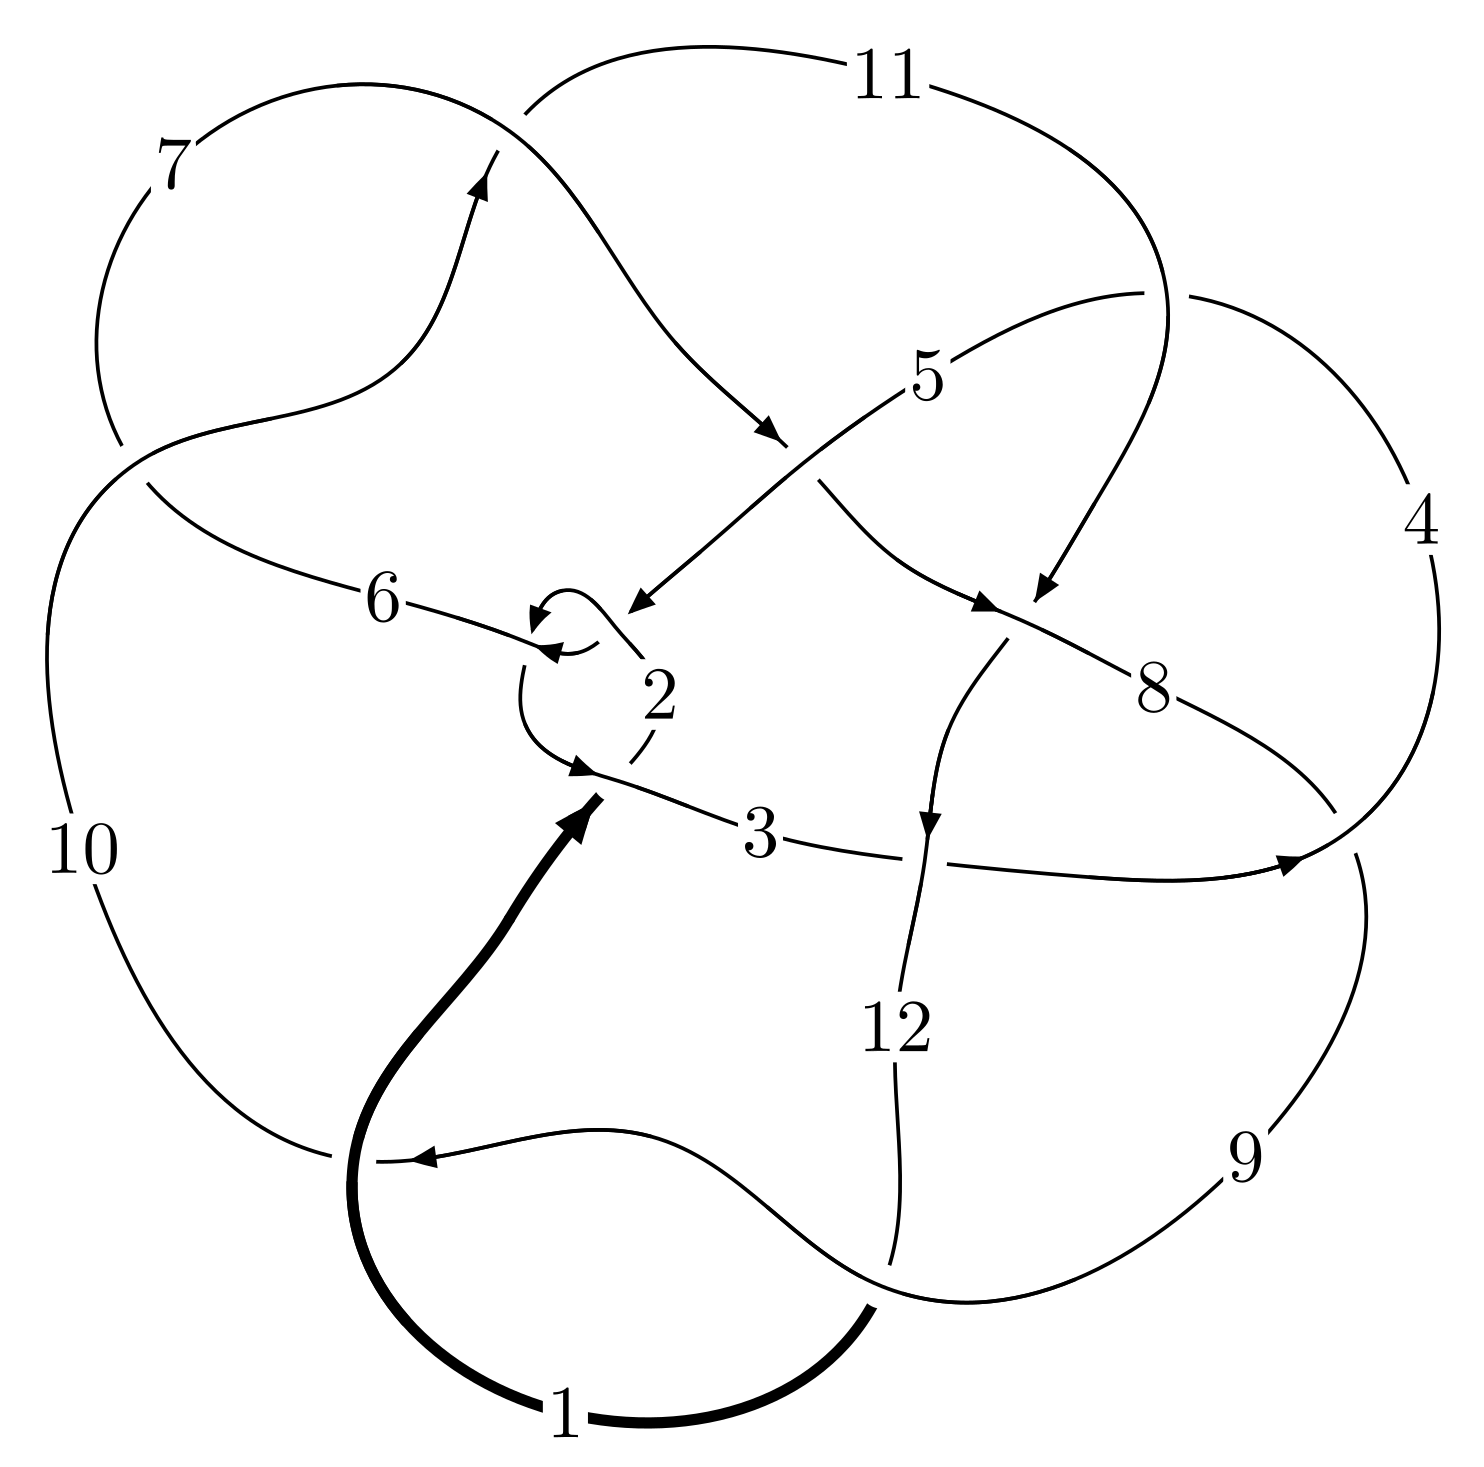
\includegraphics[width=112pt]{../../../GIT/diagram.site/Diagrams/png/1296_12a_0495.png}\\
\ \ \ A knot diagram\footnotemark}&
\allowdisplaybreaks
\textbf{Linearized knot diagam} \\
\cline{2-2}
 &
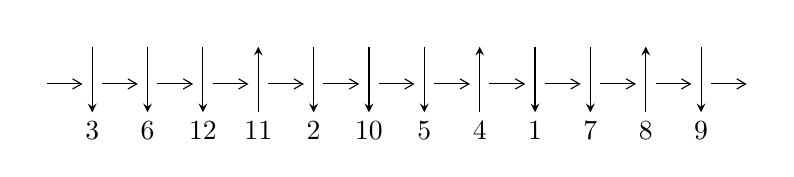
\begin{tikzpicture}[x=20pt, y=17pt]
	% nodes
	\node (C0) at (0, 0) {};
	\node (C1) at (1, 0) {};
	\node (C1U) at (1, +1) {};
	\node (C1D) at (1, -1) {3};

	\node (C2) at (2, 0) {};
	\node (C2U) at (2, +1) {};
	\node (C2D) at (2, -1) {6};

	\node (C3) at (3, 0) {};
	\node (C3U) at (3, +1) {};
	\node (C3D) at (3, -1) {12};

	\node (C4) at (4, 0) {};
	\node (C4U) at (4, +1) {};
	\node (C4D) at (4, -1) {11};

	\node (C5) at (5, 0) {};
	\node (C5U) at (5, +1) {};
	\node (C5D) at (5, -1) {2};

	\node (C6) at (6, 0) {};
	\node (C6U) at (6, +1) {};
	\node (C6D) at (6, -1) {10};

	\node (C7) at (7, 0) {};
	\node (C7U) at (7, +1) {};
	\node (C7D) at (7, -1) {5};

	\node (C8) at (8, 0) {};
	\node (C8U) at (8, +1) {};
	\node (C8D) at (8, -1) {4};

	\node (C9) at (9, 0) {};
	\node (C9U) at (9, +1) {};
	\node (C9D) at (9, -1) {1};

	\node (C10) at (10, 0) {};
	\node (C10U) at (10, +1) {};
	\node (C10D) at (10, -1) {7};

	\node (C11) at (11, 0) {};
	\node (C11U) at (11, +1) {};
	\node (C11D) at (11, -1) {8};

	\node (C12) at (12, 0) {};
	\node (C12U) at (12, +1) {};
	\node (C12D) at (12, -1) {9};
	\node (C13) at (13, 0) {};

	% arrows
	\draw[->,>={angle 60}]
	(C0) edge (C1) (C1) edge (C2) (C2) edge (C3) (C3) edge (C4) (C4) edge (C5) (C5) edge (C6) (C6) edge (C7) (C7) edge (C8) (C8) edge (C9) (C9) edge (C10) (C10) edge (C11) (C11) edge (C12) (C12) edge (C13) ;	\draw[->,>=stealth]
	(C1U) edge (C1D) (C2U) edge (C2D) (C3U) edge (C3D) (C4D) edge (C4U) (C5U) edge (C5D) (C6U) edge (C6D) (C7U) edge (C7D) (C8D) edge (C8U) (C9U) edge (C9D) (C10U) edge (C10D) (C11D) edge (C11U) (C12U) edge (C12D) ;
	\end{tikzpicture} \\
\hhline{~~} \\& 
\textbf{Solving Sequence} \\ \cline{2-2} 
 &
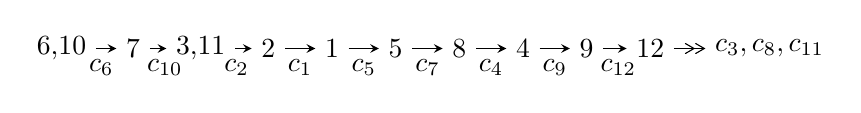
\begin{tikzpicture}[x=23pt, y=7pt]
	% node
	\node (A0) at (-1/8, 0) {6,10};
	\node (A1) at (1, 0) {7};
	\node (A2) at (33/16, 0) {3,11};
	\node (A3) at (25/8, 0) {2};
	\node (A4) at (33/8, 0) {1};
	\node (A5) at (41/8, 0) {5};
	\node (A6) at (49/8, 0) {8};
	\node (A7) at (57/8, 0) {4};
	\node (A8) at (65/8, 0) {9};
	\node (A9) at (73/8, 0) {12};
	\node (C1) at (1/2, -1) {$c_{6}$};
	\node (C2) at (3/2, -1) {$c_{10}$};
	\node (C3) at (21/8, -1) {$c_{2}$};
	\node (C4) at (29/8, -1) {$c_{1}$};
	\node (C5) at (37/8, -1) {$c_{5}$};
	\node (C6) at (45/8, -1) {$c_{7}$};
	\node (C7) at (53/8, -1) {$c_{4}$};
	\node (C8) at (61/8, -1) {$c_{9}$};
	\node (C9) at (69/8, -1) {$c_{12}$};
	\node (A10) at (11, 0) {$c_{3},c_{8},c_{11}$};

	% edge
	\draw[->,>=stealth]	
	(A0) edge (A1) (A1) edge (A2) (A2) edge (A3) (A3) edge (A4) (A4) edge (A5) (A5) edge (A6) (A6) edge (A7) (A7) edge (A8) (A8) edge (A9) ;
	\draw[->>,>={angle 60}]	
	(A9) edge (A10);
\end{tikzpicture} \\ 

\end{tabular} \\

\footnotetext{
The image of knot diagram is generated by the software ``\textbf{Draw programme}" developed by Andrew Bartholomew(\url{http://www.layer8.co.uk/maths/draw/index.htm\#Running-draw}), where we modified some parts for our purpose(\url{https://github.com/CATsTAILs/LinksPainter}).
}\phantom \\ \newline 
\centering \textbf{Ideals for irreducible components\footnotemark of $X_{\text{par}}$} 
 
\begin{align*}
I^u_{1}&=\langle 
4.50165\times10^{42} u^{42}-3.19414\times10^{44} u^{41}+\cdots+3.84773\times10^{44} b+2.85090\times10^{44},\\
\phantom{I^u_{1}}&\phantom{= \langle  }-3.52358\times10^{44} u^{42}-1.24699\times10^{44} u^{41}+\cdots+3.84773\times10^{44} a+3.72957\times10^{44},\;u^{43}+u^{42}+\cdots+2 u-1\rangle \\
I^u_{2}&=\langle 
-6.47610\times10^{471} u^{99}+1.24291\times10^{472} u^{98}+\cdots+1.82398\times10^{472} b+1.18729\times10^{475},\\
\phantom{I^u_{2}}&\phantom{= \langle  }1.09026\times10^{476} u^{99}-2.10040\times10^{476} u^{98}+\cdots+7.28496\times10^{475} a-2.02260\times10^{479},\\
\phantom{I^u_{2}}&\phantom{= \langle  }u^{100}-3 u^{99}+\cdots-14102 u+1997\rangle \\
I^u_{3}&=\langle 
b+u,\;- u^3+a+u,\;u^4+u^3- u^2- u+1\rangle \\
I^u_{4}&=\langle 
-9 u^{12}+14 u^{11}+24 u^{10}-61 u^9-18 u^8+117 u^7-19 u^6-134 u^5+56 u^4+88 u^3-58 u^2+b-36 u+19,\\
\phantom{I^u_{4}}&\phantom{= \langle  }12 u^{12}-19 u^{11}-32 u^{10}+83 u^9+23 u^8-160 u^7+29 u^6+183 u^5-80 u^4-120 u^3+82 u^2+a+48 u-27,\\
\phantom{I^u_{4}}&\phantom{= \langle  }u^{13}-2 u^{12}-2 u^{11}+8 u^{10}- u^9-14 u^8+8 u^7+14 u^6-13 u^5-7 u^4+11 u^3+u^2-4 u+1\rangle \\
I^u_{5}&=\langle 
b+1,\;a^2+a-4 u-6,\;u^2+u-1\rangle \\
\\
\end{align*}
\raggedright * 5 irreducible components of $\dim_{\mathbb{C}}=0$, with total 164 representations.\\
\footnotetext{All coefficients of polynomials are rational numbers. But the coefficients are sometimes approximated in decimal forms when there is not enough margin.}
\newpage
\renewcommand{\arraystretch}{1}
\centering \section*{I. $I^u_{1}= \langle 4.50\times10^{42} u^{42}-3.19\times10^{44} u^{41}+\cdots+3.85\times10^{44} b+2.85\times10^{44},\;-3.52\times10^{44} u^{42}-1.25\times10^{44} u^{41}+\cdots+3.85\times10^{44} a+3.73\times10^{44},\;u^{43}+u^{42}+\cdots+2 u-1 \rangle$}
\flushleft \textbf{(i) Arc colorings}\\
\begin{tabular}{m{7pt} m{180pt} m{7pt} m{180pt} }
\flushright $a_{6}=$&$\begin{pmatrix}1\\0\end{pmatrix}$ \\
\flushright $a_{10}=$&$\begin{pmatrix}0\\u\end{pmatrix}$ \\
\flushright $a_{7}=$&$\begin{pmatrix}1\\u^2\end{pmatrix}$ \\
\flushright $a_{3}=$&$\begin{pmatrix}0.915756 u^{42}+0.324085 u^{41}+\cdots-8.28487 u-0.969292\\-0.0116995 u^{42}+0.830137 u^{41}+\cdots+11.5769 u-0.740930\end{pmatrix}$ \\
\flushright $a_{11}=$&$\begin{pmatrix}- u\\- u^3+u\end{pmatrix}$ \\
\flushright $a_{2}=$&$\begin{pmatrix}0.904056 u^{42}+1.15422 u^{41}+\cdots+3.29201 u-1.71022\\-0.0116995 u^{42}+0.830137 u^{41}+\cdots+11.5769 u-0.740930\end{pmatrix}$ \\
\flushright $a_{1}=$&$\begin{pmatrix}-1\\-0.858365 u^{42}-0.500568 u^{41}+\cdots-0.685046 u+0.703287\end{pmatrix}$ \\
\flushright $a_{5}=$&$\begin{pmatrix}-0.0298597 u^{42}-0.939789 u^{41}+\cdots+24.8126 u-2.91645\\0.885896 u^{42}-0.615704 u^{41}+\cdots+16.5277 u-3.88574\end{pmatrix}$ \\
\flushright $a_{8}=$&$\begin{pmatrix}1.25763 u^{42}+0.566937 u^{41}+\cdots+7.76709 u+0.365042\\-0.359305 u^{42}+0.0358520 u^{41}+\cdots+1.77109 u+0.0735383\end{pmatrix}$ \\
\flushright $a_{4}=$&$\begin{pmatrix}-0.535897 u^{42}+0.224628 u^{41}+\cdots+20.0722 u-1.23522\\0.624186 u^{42}-0.362368 u^{41}+\cdots+17.4211 u-3.89651\end{pmatrix}$ \\
\flushright $a_{9}=$&$\begin{pmatrix}u\\-0.357797 u^{42}+0.447881 u^{41}+\cdots-1.42002 u+0.858365\end{pmatrix}$ \\
\flushright $a_{12}=$&$\begin{pmatrix}u^2-1\\-0.0526870 u^{42}-0.367362 u^{41}+\cdots+0.888912 u+0.345490\end{pmatrix}$\\&\end{tabular}
\flushleft \textbf{(ii) Obstruction class $= -1$}\\~\\
\flushleft \textbf{(iii) Cusp Shapes $= -2.11254 u^{42}+0.229872 u^{41}+\cdots-39.9613 u-5.19110$}\\~\\
\newpage\renewcommand{\arraystretch}{1}
\flushleft \textbf{(iv) u-Polynomials at the component}\newline \\
\begin{tabular}{m{50pt}|m{274pt}}
Crossings & \hspace{64pt}u-Polynomials at each crossing \\
\hline $$\begin{aligned}c_{1}\end{aligned}$$&$\begin{aligned}
&u^{43}+18 u^{42}+\cdots+6320 u+256
\end{aligned}$\\
\hline $$\begin{aligned}c_{2},c_{5}\end{aligned}$$&$\begin{aligned}
&u^{43}+12 u^{42}+\cdots+204 u+16
\end{aligned}$\\
\hline $$\begin{aligned}c_{3},c_{7}\end{aligned}$$&$\begin{aligned}
&u^{43}-2 u^{42}+\cdots-11 u+1
\end{aligned}$\\
\hline $$\begin{aligned}c_{4},c_{8}\end{aligned}$$&$\begin{aligned}
&u^{43}+15 u^{41}+\cdots+3 u+1
\end{aligned}$\\
\hline $$\begin{aligned}c_{6},c_{9},c_{10}\\c_{12}\end{aligned}$$&$\begin{aligned}
&u^{43}- u^{42}+\cdots+2 u+1
\end{aligned}$\\
\hline $$\begin{aligned}c_{11}\end{aligned}$$&$\begin{aligned}
&u^{43}-18 u^{42}+\cdots+8 u+4
\end{aligned}$\\
\hline
\end{tabular}\\~\\
\newpage\renewcommand{\arraystretch}{1}
\flushleft \textbf{(v) Riley Polynomials at the component}\newline \\
\begin{tabular}{m{50pt}|m{274pt}}
Crossings & \hspace{64pt}Riley Polynomials at each crossing \\
\hline $$\begin{aligned}c_{1}\end{aligned}$$&$\begin{aligned}
&y^{43}+18 y^{42}+\cdots+23099136 y-65536
\end{aligned}$\\
\hline $$\begin{aligned}c_{2},c_{5}\end{aligned}$$&$\begin{aligned}
&y^{43}-18 y^{42}+\cdots+6320 y-256
\end{aligned}$\\
\hline $$\begin{aligned}c_{3},c_{7}\end{aligned}$$&$\begin{aligned}
&y^{43}+2 y^{42}+\cdots+49 y-1
\end{aligned}$\\
\hline $$\begin{aligned}c_{4},c_{8}\end{aligned}$$&$\begin{aligned}
&y^{43}+30 y^{42}+\cdots-51 y-1
\end{aligned}$\\
\hline $$\begin{aligned}c_{6},c_{9},c_{10}\\c_{12}\end{aligned}$$&$\begin{aligned}
&y^{43}-41 y^{42}+\cdots+60 y-1
\end{aligned}$\\
\hline $$\begin{aligned}c_{11}\end{aligned}$$&$\begin{aligned}
&y^{43}-6 y^{42}+\cdots+168 y-16
\end{aligned}$\\
\hline
\end{tabular}\\~\\
\newpage\flushleft \textbf{(vi) Complex Volumes and Cusp Shapes}
$$\begin{array}{c|c|c}  
\text{Solutions to }I^u_{1}& \I (\text{vol} + \sqrt{-1}CS) & \text{Cusp shape}\\
 \hline 
\begin{aligned}
u &= -0.117499 + 1.004120 I \\
a &= -0.503747 + 1.230070 I \\
b &= \phantom{-}0.714886 - 0.696202 I\end{aligned}
 & \phantom{-}3.79723 - 2.80030 I & -1.75451 + 2.24956 I \\ \hline\begin{aligned}
u &= -0.117499 - 1.004120 I \\
a &= -0.503747 - 1.230070 I \\
b &= \phantom{-}0.714886 + 0.696202 I\end{aligned}
 & \phantom{-}3.79723 + 2.80030 I & -1.75451 - 2.24956 I \\ \hline\begin{aligned}
u &= \phantom{-}0.062916 + 1.011790 I \\
a &= -0.15608 - 1.47247 I \\
b &= \phantom{-}0.928815 + 0.671587 I\end{aligned}
 & \phantom{-}3.17076 - 8.04245 I & -3.44286 + 8.35826 I \\ \hline\begin{aligned}
u &= \phantom{-}0.062916 - 1.011790 I \\
a &= -0.15608 + 1.47247 I \\
b &= \phantom{-}0.928815 - 0.671587 I\end{aligned}
 & \phantom{-}3.17076 + 8.04245 I & -3.44286 - 8.35826 I \\ \hline\begin{aligned}
u &= \phantom{-}1.069580 + 0.138287 I \\
a &= \phantom{-}0.792890 - 1.128880 I \\
b &= \phantom{-}1.41664 + 0.59320 I\end{aligned}
 & -6.25292 - 1.45389 I & -15.9994 - 2.3137 I \\ \hline\begin{aligned}
u &= \phantom{-}1.069580 - 0.138287 I \\
a &= \phantom{-}0.792890 + 1.128880 I \\
b &= \phantom{-}1.41664 - 0.59320 I\end{aligned}
 & -6.25292 + 1.45389 I & -15.9994 + 2.3137 I \\ \hline\begin{aligned}
u &= \phantom{-}1.109200 + 0.079633 I \\
a &= -0.211055 - 0.682003 I \\
b &= \phantom{-}0.58590 + 1.33812 I\end{aligned}
 & -2.84647 - 6.20636 I & -11.78082 + 7.78840 I \\ \hline\begin{aligned}
u &= \phantom{-}1.109200 - 0.079633 I \\
a &= -0.211055 + 0.682003 I \\
b &= \phantom{-}0.58590 - 1.33812 I\end{aligned}
 & -2.84647 + 6.20636 I & -11.78082 - 7.78840 I \\ \hline\begin{aligned}
u &= \phantom{-}0.912089 + 0.720865 I \\
a &= -0.10294 - 1.89195 I \\
b &= \phantom{-}0.971326 + 0.526994 I\end{aligned}
 & -1.90367 - 3.73876 I & -5.13722 + 7.22741 I \\ \hline\begin{aligned}
u &= \phantom{-}0.912089 - 0.720865 I \\
a &= -0.10294 + 1.89195 I \\
b &= \phantom{-}0.971326 - 0.526994 I\end{aligned}
 & -1.90367 + 3.73876 I & -5.13722 - 7.22741 I\\
 \hline 
 \end{array}$$\newpage$$\begin{array}{c|c|c}  
\text{Solutions to }I^u_{1}& \I (\text{vol} + \sqrt{-1}CS) & \text{Cusp shape}\\
 \hline 
\begin{aligned}
u &= -1.185440 + 0.005135 I \\
a &= -0.504645 - 0.907568 I \\
b &= \phantom{-}0.532020 + 0.841629 I\end{aligned}
 & -5.72482 - 1.57132 I & -12.72131 + 2.39726 I \\ \hline\begin{aligned}
u &= -1.185440 - 0.005135 I \\
a &= -0.504645 + 0.907568 I \\
b &= \phantom{-}0.532020 - 0.841629 I\end{aligned}
 & -5.72482 + 1.57132 I & -12.72131 - 2.39726 I \\ \hline\begin{aligned}
u &= -1.218930 + 0.142311 I \\
a &= \phantom{-}0.234566 + 0.991044 I \\
b &= \phantom{-}1.22616 - 0.95551 I\end{aligned}
 & -5.77798 + 4.07207 I & -16.1651 - 7.5060 I \\ \hline\begin{aligned}
u &= -1.218930 - 0.142311 I \\
a &= \phantom{-}0.234566 - 0.991044 I \\
b &= \phantom{-}1.22616 + 0.95551 I\end{aligned}
 & -5.77798 - 4.07207 I & -16.1651 + 7.5060 I \\ \hline\begin{aligned}
u &= -1.243430 + 0.252908 I \\
a &= \phantom{-}0.16597 + 1.57644 I \\
b &= \phantom{-}1.066050 - 0.627388 I\end{aligned}
 & -7.37478 + 3.89701 I & -14.05829 + 0. I\phantom{ +0.000000I} \\ \hline\begin{aligned}
u &= -1.243430 - 0.252908 I \\
a &= \phantom{-}0.16597 - 1.57644 I \\
b &= \phantom{-}1.066050 + 0.627388 I\end{aligned}
 & -7.37478 - 3.89701 I & -14.05829 + 0. I\phantom{ +0.000000I} \\ \hline\begin{aligned}
u &= \phantom{-}0.481551 + 0.543549 I \\
a &= -0.95293 + 1.62097 I \\
b &= \phantom{-}0.730477 - 0.458470 I\end{aligned}
 & -1.010270 + 0.399925 I & -5.75032 + 1.08841 I \\ \hline\begin{aligned}
u &= \phantom{-}0.481551 - 0.543549 I \\
a &= -0.95293 - 1.62097 I \\
b &= \phantom{-}0.730477 + 0.458470 I\end{aligned}
 & -1.010270 - 0.399925 I & -5.75032 - 1.08841 I \\ \hline\begin{aligned}
u &= \phantom{-}0.661900\phantom{ +0.000000I} \\
a &= -1.30419\phantom{ +0.000000I} \\
b &= \phantom{-}0.233241\phantom{ +0.000000I}\end{aligned}
 & -1.19793\phantom{ +0.000000I} & -7.72930\phantom{ +0.000000I} \\ \hline\begin{aligned}
u &= \phantom{-}0.019937 + 0.656213 I \\
a &= -0.520963 + 0.051706 I \\
b &= -0.900796 - 0.188656 I\end{aligned}
 & -1.62331 - 3.89803 I & -10.31136 + 7.16780 I\\
 \hline 
 \end{array}$$\newpage$$\begin{array}{c|c|c}  
\text{Solutions to }I^u_{1}& \I (\text{vol} + \sqrt{-1}CS) & \text{Cusp shape}\\
 \hline 
\begin{aligned}
u &= \phantom{-}0.019937 - 0.656213 I \\
a &= -0.520963 - 0.051706 I \\
b &= -0.900796 + 0.188656 I\end{aligned}
 & -1.62331 + 3.89803 I & -10.31136 - 7.16780 I \\ \hline\begin{aligned}
u &= \phantom{-}1.362940 + 0.240786 I \\
a &= -0.500176 - 0.102046 I \\
b &= -0.919402 + 0.391596 I\end{aligned}
 & -2.88611 + 1.54391 I & \phantom{-0.000000 } 0 \\ \hline\begin{aligned}
u &= \phantom{-}1.362940 - 0.240786 I \\
a &= -0.500176 + 0.102046 I \\
b &= -0.919402 - 0.391596 I\end{aligned}
 & -2.88611 - 1.54391 I & \phantom{-0.000000 } 0 \\ \hline\begin{aligned}
u &= -0.259331 + 0.529204 I \\
a &= -0.758126 - 0.463356 I \\
b &= \phantom{-}0.039682 + 0.586932 I\end{aligned}
 & \phantom{-}1.26738 - 1.62023 I & \phantom{-}0.40000 + 1.60958 I \\ \hline\begin{aligned}
u &= -0.259331 - 0.529204 I \\
a &= -0.758126 + 0.463356 I \\
b &= \phantom{-}0.039682 - 0.586932 I\end{aligned}
 & \phantom{-}1.26738 + 1.62023 I & \phantom{-}0.40000 - 1.60958 I \\ \hline\begin{aligned}
u &= \phantom{-}1.40146 + 0.24459 I \\
a &= -0.412623 - 0.005640 I \\
b &= -1.42306 + 0.03312 I\end{aligned}
 & -11.2007 - 10.2230 I & \phantom{-0.000000 } 0 \\ \hline\begin{aligned}
u &= \phantom{-}1.40146 - 0.24459 I \\
a &= -0.412623 + 0.005640 I \\
b &= -1.42306 - 0.03312 I\end{aligned}
 & -11.2007 + 10.2230 I & \phantom{-0.000000 } 0 \\ \hline\begin{aligned}
u &= -1.35615 + 0.48076 I \\
a &= -0.501656 - 0.811085 I \\
b &= \phantom{-}0.448437 + 0.891775 I\end{aligned}
 & -6.31477 + 5.74152 I & \phantom{-0.000000 } 0 \\ \hline\begin{aligned}
u &= -1.35615 - 0.48076 I \\
a &= -0.501656 + 0.811085 I \\
b &= \phantom{-}0.448437 - 0.891775 I\end{aligned}
 & -6.31477 - 5.74152 I & \phantom{-0.000000 } 0 \\ \hline\begin{aligned}
u &= \phantom{-}1.37918 + 0.51314 I \\
a &= -0.415180 + 0.729199 I \\
b &= \phantom{-}0.410344 - 1.035640 I\end{aligned}
 & -4.2607 - 13.9202 I & \phantom{-0.000000 } 0\\
 \hline 
 \end{array}$$\newpage$$\begin{array}{c|c|c}  
\text{Solutions to }I^u_{1}& \I (\text{vol} + \sqrt{-1}CS) & \text{Cusp shape}\\
 \hline 
\begin{aligned}
u &= \phantom{-}1.37918 - 0.51314 I \\
a &= -0.415180 - 0.729199 I \\
b &= \phantom{-}0.410344 + 1.035640 I\end{aligned}
 & -4.2607 + 13.9202 I & \phantom{-0.000000 } 0 \\ \hline\begin{aligned}
u &= -1.51469 + 0.21936 I \\
a &= -0.447254 + 0.012516 I \\
b &= -1.234120 - 0.062522 I\end{aligned}
 & -12.36260 + 3.19642 I & \phantom{-0.000000 } 0 \\ \hline\begin{aligned}
u &= -1.51469 - 0.21936 I \\
a &= -0.447254 - 0.012516 I \\
b &= -1.234120 + 0.062522 I\end{aligned}
 & -12.36260 - 3.19642 I & \phantom{-0.000000 } 0 \\ \hline\begin{aligned}
u &= -1.46914 + 0.59124 I \\
a &= \phantom{-}0.30263 + 1.47349 I \\
b &= \phantom{-}1.133750 - 0.651193 I\end{aligned}
 & -8.4013 + 11.4319 I & \phantom{-0.000000 } 0 \\ \hline\begin{aligned}
u &= -1.46914 - 0.59124 I \\
a &= \phantom{-}0.30263 - 1.47349 I \\
b &= \phantom{-}1.133750 + 0.651193 I\end{aligned}
 & -8.4013 - 11.4319 I & \phantom{-0.000000 } 0 \\ \hline\begin{aligned}
u &= \phantom{-}1.49429 + 0.58038 I \\
a &= \phantom{-}0.396103 - 1.357230 I \\
b &= \phantom{-}1.198150 + 0.678964 I\end{aligned}
 & -6.7222 - 20.0860 I & \phantom{-0.000000 } 0 \\ \hline\begin{aligned}
u &= \phantom{-}1.49429 - 0.58038 I \\
a &= \phantom{-}0.396103 + 1.357230 I \\
b &= \phantom{-}1.198150 - 0.678964 I\end{aligned}
 & -6.7222 + 20.0860 I & \phantom{-0.000000 } 0 \\ \hline\begin{aligned}
u &= -1.73149 + 0.11092 I \\
a &= -0.507401 + 0.093242 I \\
b &= -0.906448 - 0.350335 I\end{aligned}
 & -9.79548 - 1.45521 I & \phantom{-0.000000 } 0 \\ \hline\begin{aligned}
u &= -1.73149 - 0.11092 I \\
a &= -0.507401 - 0.093242 I \\
b &= -0.906448 + 0.350335 I\end{aligned}
 & -9.79548 + 1.45521 I & \phantom{-0.000000 } 0 \\ \hline\begin{aligned}
u &= -0.247184 + 0.021411 I \\
a &= -0.440997 + 0.191569 I \\
b &= -0.907616 - 0.828669 I\end{aligned}
 & \phantom{-}4.28256 - 3.09500 I & \phantom{-}12.20187 - 2.50782 I\\
 \hline 
 \end{array}$$\newpage$$\begin{array}{c|c|c}  
\text{Solutions to }I^u_{1}& \I (\text{vol} + \sqrt{-1}CS) & \text{Cusp shape}\\
 \hline 
\begin{aligned}
u &= -0.247184 - 0.021411 I \\
a &= -0.440997 - 0.191569 I \\
b &= -0.907616 + 0.828669 I\end{aligned}
 & \phantom{-}4.28256 + 3.09500 I & \phantom{-}12.20187 + 2.50782 I \\ \hline\begin{aligned}
u &= \phantom{-}0.219210 + 0.092274 I \\
a &= -3.80430 - 1.49216 I \\
b &= \phantom{-}0.772188 + 0.089355 I\end{aligned}
 & -1.352550 - 0.324869 I & -8.63286 + 1.59353 I \\ \hline\begin{aligned}
u &= \phantom{-}0.219210 - 0.092274 I \\
a &= -3.80430 + 1.49216 I \\
b &= \phantom{-}0.772188 - 0.089355 I\end{aligned}
 & -1.352550 + 0.324869 I & -8.63286 - 1.59353 I\\
 \hline 
 \end{array}$$\newpage\newpage\renewcommand{\arraystretch}{1}
\centering \section*{II. $I^u_{2}= \langle -6.48\times10^{471} u^{99}+1.24\times10^{472} u^{98}+\cdots+1.82\times10^{472} b+1.19\times10^{475},\;1.09\times10^{476} u^{99}-2.10\times10^{476} u^{98}+\cdots+7.28\times10^{475} a-2.02\times10^{479},\;u^{100}-3 u^{99}+\cdots-14102 u+1997 \rangle$}
\flushleft \textbf{(i) Arc colorings}\\
\begin{tabular}{m{7pt} m{180pt} m{7pt} m{180pt} }
\flushright $a_{6}=$&$\begin{pmatrix}1\\0\end{pmatrix}$ \\
\flushright $a_{10}=$&$\begin{pmatrix}0\\u\end{pmatrix}$ \\
\flushright $a_{7}=$&$\begin{pmatrix}1\\u^2\end{pmatrix}$ \\
\flushright $a_{3}=$&$\begin{pmatrix}-1.49660 u^{99}+2.88319 u^{98}+\cdots-17051.6 u+2776.40\\0.355054 u^{99}-0.681427 u^{98}+\cdots+4015.19 u-650.934\end{pmatrix}$ \\
\flushright $a_{11}=$&$\begin{pmatrix}- u\\- u^3+u\end{pmatrix}$ \\
\flushright $a_{2}=$&$\begin{pmatrix}-1.14154 u^{99}+2.20177 u^{98}+\cdots-13036.4 u+2125.46\\0.355054 u^{99}-0.681427 u^{98}+\cdots+4015.19 u-650.934\end{pmatrix}$ \\
\flushright $a_{1}=$&$\begin{pmatrix}-1.72142 u^{99}+3.30112 u^{98}+\cdots-19491.2 u+3175.97\\-0.513029 u^{99}+0.985355 u^{98}+\cdots-5825.26 u+951.619\end{pmatrix}$ \\
\flushright $a_{5}=$&$\begin{pmatrix}0.00681558 u^{99}+0.000928500 u^{98}+\cdots-46.7083 u+11.5955\\0.622392 u^{99}-1.20360 u^{98}+\cdots+7159.72 u-1172.37\end{pmatrix}$ \\
\flushright $a_{8}=$&$\begin{pmatrix}-1.19879 u^{99}+2.31683 u^{98}+\cdots-13648.7 u+2220.10\\1.51223 u^{99}-2.88894 u^{98}+\cdots+16991.6 u-2762.04\end{pmatrix}$ \\
\flushright $a_{4}=$&$\begin{pmatrix}-0.666675 u^{99}+1.30122 u^{98}+\cdots-7754.81 u+1270.54\\0.525452 u^{99}-1.01692 u^{98}+\cdots+6056.80 u-993.112\end{pmatrix}$ \\
\flushright $a_{9}=$&$\begin{pmatrix}-0.793074 u^{99}+1.54287 u^{98}+\cdots-9165.38 u+1507.47\\1.29836 u^{99}-2.48147 u^{98}+\cdots+14600.4 u-2373.20\end{pmatrix}$ \\
\flushright $a_{12}=$&$\begin{pmatrix}-15.2590 u^{99}+29.3676 u^{98}+\cdots-173710. u+28330.9\\-2.90740 u^{99}+5.60560 u^{98}+\cdots-33193.5 u+5412.75\end{pmatrix}$\\&\end{tabular}
\flushleft \textbf{(ii) Obstruction class $= -1$}\\~\\
\flushleft \textbf{(iii) Cusp Shapes $= -20.4788 u^{99}+39.2181 u^{98}+\cdots-231611. u+37764.1$}\\~\\
\newpage\renewcommand{\arraystretch}{1}
\flushleft \textbf{(iv) u-Polynomials at the component}\newline \\
\begin{tabular}{m{50pt}|m{274pt}}
Crossings & \hspace{64pt}u-Polynomials at each crossing \\
\hline $$\begin{aligned}c_{1}\end{aligned}$$&$\begin{aligned}
&(u^{50}+24 u^{49}+\cdots+50 u+1)^{2}
\end{aligned}$\\
\hline $$\begin{aligned}c_{2},c_{5}\end{aligned}$$&$\begin{aligned}
&(u^{50}-4 u^{49}+\cdots+6 u+1)^{2}
\end{aligned}$\\
\hline $$\begin{aligned}c_{3},c_{7}\end{aligned}$$&$\begin{aligned}
&u^{100}-8 u^{99}+\cdots+35 u-1
\end{aligned}$\\
\hline $$\begin{aligned}c_{4},c_{8}\end{aligned}$$&$\begin{aligned}
&u^{100}-2 u^{99}+\cdots+1541 u-1189
\end{aligned}$\\
\hline $$\begin{aligned}c_{6},c_{9},c_{10}\\c_{12}\end{aligned}$$&$\begin{aligned}
&u^{100}+3 u^{99}+\cdots+14102 u+1997
\end{aligned}$\\
\hline $$\begin{aligned}c_{11}\end{aligned}$$&$\begin{aligned}
&(u^{50}+12 u^{49}+\cdots+16 u-4)^{2}
\end{aligned}$\\
\hline
\end{tabular}\\~\\
\newpage\renewcommand{\arraystretch}{1}
\flushleft \textbf{(v) Riley Polynomials at the component}\newline \\
\begin{tabular}{m{50pt}|m{274pt}}
Crossings & \hspace{64pt}Riley Polynomials at each crossing \\
\hline $$\begin{aligned}c_{1}\end{aligned}$$&$\begin{aligned}
&(y^{50}+4 y^{48}+\cdots-10 y+1)^{2}
\end{aligned}$\\
\hline $$\begin{aligned}c_{2},c_{5}\end{aligned}$$&$\begin{aligned}
&(y^{50}-24 y^{49}+\cdots-50 y+1)^{2}
\end{aligned}$\\
\hline $$\begin{aligned}c_{3},c_{7}\end{aligned}$$&$\begin{aligned}
&y^{100}-10 y^{99}+\cdots-161 y+1
\end{aligned}$\\
\hline $$\begin{aligned}c_{4},c_{8}\end{aligned}$$&$\begin{aligned}
&y^{100}+2 y^{99}+\cdots+65873919 y+1413721
\end{aligned}$\\
\hline $$\begin{aligned}c_{6},c_{9},c_{10}\\c_{12}\end{aligned}$$&$\begin{aligned}
&y^{100}-63 y^{99}+\cdots-99531630 y+3988009
\end{aligned}$\\
\hline $$\begin{aligned}c_{11}\end{aligned}$$&$\begin{aligned}
&(y^{50}-6 y^{49}+\cdots-360 y+16)^{2}
\end{aligned}$\\
\hline
\end{tabular}\\~\\
\newpage\flushleft \textbf{(vi) Complex Volumes and Cusp Shapes}
$$\begin{array}{c|c|c}  
\text{Solutions to }I^u_{2}& \I (\text{vol} + \sqrt{-1}CS) & \text{Cusp shape}\\
 \hline 
\begin{aligned}
u &= \phantom{-}0.656763 + 0.760795 I \\
a &= -0.584932 + 1.144110 I \\
b &= -0.436168 - 0.694869 I\end{aligned}
 & \phantom{-}0.427144 + 1.052320 I & \phantom{-0.000000 } 0 \\ \hline\begin{aligned}
u &= \phantom{-}0.656763 - 0.760795 I \\
a &= -0.584932 - 1.144110 I \\
b &= -0.436168 + 0.694869 I\end{aligned}
 & \phantom{-}0.427144 - 1.052320 I & \phantom{-0.000000 } 0 \\ \hline\begin{aligned}
u &= \phantom{-}0.905026 + 0.412300 I \\
a &= \phantom{-}0.550286 - 0.702215 I \\
b &= -0.216437 + 1.063560 I\end{aligned}
 & -0.47368 - 5.62173 I & \phantom{-0.000000 } 0 \\ \hline\begin{aligned}
u &= \phantom{-}0.905026 - 0.412300 I \\
a &= \phantom{-}0.550286 + 0.702215 I \\
b &= -0.216437 - 1.063560 I\end{aligned}
 & -0.47368 + 5.62173 I & \phantom{-0.000000 } 0 \\ \hline\begin{aligned}
u &= \phantom{-}0.949536 + 0.348439 I \\
a &= -1.218050 - 0.554976 I \\
b &= \phantom{-}0.745385 - 0.169931 I\end{aligned}
 & -2.44170 - 0.46878 I & \phantom{-0.000000 } 0 \\ \hline\begin{aligned}
u &= \phantom{-}0.949536 - 0.348439 I \\
a &= -1.218050 + 0.554976 I \\
b &= \phantom{-}0.745385 + 0.169931 I\end{aligned}
 & -2.44170 + 0.46878 I & \phantom{-0.000000 } 0 \\ \hline\begin{aligned}
u &= \phantom{-}1.011970 + 0.097016 I \\
a &= \phantom{-}1.53769 + 1.22745 I \\
b &= -0.736456 - 0.667448 I\end{aligned}
 & -3.13684 - 2.46798 I & \phantom{-0.000000 } 0 \\ \hline\begin{aligned}
u &= \phantom{-}1.011970 - 0.097016 I \\
a &= \phantom{-}1.53769 - 1.22745 I \\
b &= -0.736456 + 0.667448 I\end{aligned}
 & -3.13684 + 2.46798 I & \phantom{-0.000000 } 0 \\ \hline\begin{aligned}
u &= \phantom{-}0.085664 + 0.965920 I \\
a &= \phantom{-}0.582554 + 1.103620 I \\
b &= -1.071100 - 0.607580 I\end{aligned}
 & \phantom{-}1.01570 - 6.59278 I & \phantom{-0.000000 } 0 \\ \hline\begin{aligned}
u &= \phantom{-}0.085664 - 0.965920 I \\
a &= \phantom{-}0.582554 - 1.103620 I \\
b &= -1.071100 + 0.607580 I\end{aligned}
 & \phantom{-}1.01570 + 6.59278 I & \phantom{-0.000000 } 0\\
 \hline 
 \end{array}$$\newpage$$\begin{array}{c|c|c}  
\text{Solutions to }I^u_{2}& \I (\text{vol} + \sqrt{-1}CS) & \text{Cusp shape}\\
 \hline 
\begin{aligned}
u &= -0.860385 + 0.444729 I \\
a &= \phantom{-}0.412609 + 0.215003 I \\
b &= -0.477882 - 0.757790 I\end{aligned}
 & \phantom{-}2.77810 + 1.41692 I & \phantom{-0.000000 } 0 \\ \hline\begin{aligned}
u &= -0.860385 - 0.444729 I \\
a &= \phantom{-}0.412609 - 0.215003 I \\
b &= -0.477882 + 0.757790 I\end{aligned}
 & \phantom{-}2.77810 - 1.41692 I & \phantom{-0.000000 } 0 \\ \hline\begin{aligned}
u &= \phantom{-}0.917557 + 0.116065 I \\
a &= -0.23436 + 2.21973 I \\
b &= -0.864244 + 0.414490 I\end{aligned}
 & -3.16942 + 1.80253 I & \phantom{-0.000000 } 0 \\ \hline\begin{aligned}
u &= \phantom{-}0.917557 - 0.116065 I \\
a &= -0.23436 - 2.21973 I \\
b &= -0.864244 - 0.414490 I\end{aligned}
 & -3.16942 - 1.80253 I & \phantom{-0.000000 } 0 \\ \hline\begin{aligned}
u &= \phantom{-}1.077360 + 0.004053 I \\
a &= -2.55658 + 2.06259 I \\
b &= -0.956692 - 0.490395 I\end{aligned}
 & -3.53615 - 1.92255 I & \phantom{-0.000000 } 0 \\ \hline\begin{aligned}
u &= \phantom{-}1.077360 - 0.004053 I \\
a &= -2.55658 - 2.06259 I \\
b &= -0.956692 + 0.490395 I\end{aligned}
 & -3.53615 + 1.92255 I & \phantom{-0.000000 } 0 \\ \hline\begin{aligned}
u &= \phantom{-}1.054110 + 0.264782 I \\
a &= -0.436059 - 0.507688 I \\
b &= \phantom{-}0.174912 - 0.072012 I\end{aligned}
 & -2.25288 - 0.54027 I & \phantom{-0.000000 } 0 \\ \hline\begin{aligned}
u &= \phantom{-}1.054110 - 0.264782 I \\
a &= -0.436059 + 0.507688 I \\
b &= \phantom{-}0.174912 + 0.072012 I\end{aligned}
 & -2.25288 + 0.54027 I & \phantom{-0.000000 } 0 \\ \hline\begin{aligned}
u &= -1.079740 + 0.178850 I \\
a &= -1.97577 + 0.70292 I \\
b &= -0.953268 - 0.231057 I\end{aligned}
 & -4.08289 + 7.09407 I & \phantom{-0.000000 } 0 \\ \hline\begin{aligned}
u &= -1.079740 - 0.178850 I \\
a &= -1.97577 - 0.70292 I \\
b &= -0.953268 + 0.231057 I\end{aligned}
 & -4.08289 - 7.09407 I & \phantom{-0.000000 } 0\\
 \hline 
 \end{array}$$\newpage$$\begin{array}{c|c|c}  
\text{Solutions to }I^u_{2}& \I (\text{vol} + \sqrt{-1}CS) & \text{Cusp shape}\\
 \hline 
\begin{aligned}
u &= -1.114640 + 0.127526 I \\
a &= \phantom{-}0.882490 - 0.625320 I \\
b &= \phantom{-}1.178820 + 0.412170 I\end{aligned}
 & -4.49981 + 0.63122 I & \phantom{-0.000000 } 0 \\ \hline\begin{aligned}
u &= -1.114640 - 0.127526 I \\
a &= \phantom{-}0.882490 + 0.625320 I \\
b &= \phantom{-}1.178820 - 0.412170 I\end{aligned}
 & -4.49981 - 0.63122 I & \phantom{-0.000000 } 0 \\ \hline\begin{aligned}
u &= \phantom{-}1.12635\phantom{ +0.000000I} \\
a &= \phantom{-}0.310968\phantom{ +0.000000I} \\
b &= \phantom{-}1.67865\phantom{ +0.000000I}\end{aligned}
 & -7.24677\phantom{ +0.000000I} & \phantom{-0.000000 } 0 \\ \hline\begin{aligned}
u &= \phantom{-}1.123620 + 0.082110 I \\
a &= \phantom{-}1.35965 - 1.86945 I \\
b &= \phantom{-}1.023230 + 0.261071 I\end{aligned}
 & -3.65706 - 0.80100 I & \phantom{-0.000000 } 0 \\ \hline\begin{aligned}
u &= \phantom{-}1.123620 - 0.082110 I \\
a &= \phantom{-}1.35965 + 1.86945 I \\
b &= \phantom{-}1.023230 - 0.261071 I\end{aligned}
 & -3.65706 + 0.80100 I & \phantom{-0.000000 } 0 \\ \hline\begin{aligned}
u &= -0.057481 + 1.129840 I \\
a &= \phantom{-}0.027247 - 1.409620 I \\
b &= \phantom{-}0.513461 + 0.735910 I\end{aligned}
 & \phantom{-}0.25096 + 8.19403 I & \phantom{-0.000000 } 0 \\ \hline\begin{aligned}
u &= -0.057481 - 1.129840 I \\
a &= \phantom{-}0.027247 + 1.409620 I \\
b &= \phantom{-}0.513461 - 0.735910 I\end{aligned}
 & \phantom{-}0.25096 - 8.19403 I & \phantom{-0.000000 } 0 \\ \hline\begin{aligned}
u &= \phantom{-}0.495922 + 1.020730 I \\
a &= \phantom{-}0.594511 - 0.531595 I \\
b &= -1.078350 + 0.573559 I\end{aligned}
 & -1.46179 + 5.95154 I & \phantom{-0.000000 } 0 \\ \hline\begin{aligned}
u &= \phantom{-}0.495922 - 1.020730 I \\
a &= \phantom{-}0.594511 + 0.531595 I \\
b &= -1.078350 - 0.573559 I\end{aligned}
 & -1.46179 - 5.95154 I & \phantom{-0.000000 } 0 \\ \hline\begin{aligned}
u &= -1.083500 + 0.384657 I \\
a &= \phantom{-}0.178705 + 0.589391 I \\
b &= \phantom{-}0.215012 - 0.897652 I\end{aligned}
 & -1.01117 + 5.33279 I & \phantom{-0.000000 } 0\\
 \hline 
 \end{array}$$\newpage$$\begin{array}{c|c|c}  
\text{Solutions to }I^u_{2}& \I (\text{vol} + \sqrt{-1}CS) & \text{Cusp shape}\\
 \hline 
\begin{aligned}
u &= -1.083500 - 0.384657 I \\
a &= \phantom{-}0.178705 - 0.589391 I \\
b &= \phantom{-}0.215012 + 0.897652 I\end{aligned}
 & -1.01117 - 5.33279 I & \phantom{-0.000000 } 0 \\ \hline\begin{aligned}
u &= -0.552128 + 0.595910 I \\
a &= \phantom{-}0.72315 + 2.39951 I \\
b &= \phantom{-}0.745385 - 0.169931 I\end{aligned}
 & -2.44170 - 0.46878 I & \phantom{-0.000000 } 0 \\ \hline\begin{aligned}
u &= -0.552128 - 0.595910 I \\
a &= \phantom{-}0.72315 - 2.39951 I \\
b &= \phantom{-}0.745385 + 0.169931 I\end{aligned}
 & -2.44170 + 0.46878 I & \phantom{-0.000000 } 0 \\ \hline\begin{aligned}
u &= -1.125100 + 0.381707 I \\
a &= -0.83288 - 1.21807 I \\
b &= -1.071100 + 0.607580 I\end{aligned}
 & \phantom{-}1.01570 + 6.59278 I & \phantom{-0.000000 } 0 \\ \hline\begin{aligned}
u &= -1.125100 - 0.381707 I \\
a &= -0.83288 + 1.21807 I \\
b &= -1.071100 - 0.607580 I\end{aligned}
 & \phantom{-}1.01570 - 6.59278 I & \phantom{-0.000000 } 0 \\ \hline\begin{aligned}
u &= -1.198300 + 0.018491 I \\
a &= \phantom{-}0.731188 + 0.480247 I \\
b &= -0.325073 - 0.850938 I\end{aligned}
 & -5.49087 + 5.13720 I & \phantom{-0.000000 } 0 \\ \hline\begin{aligned}
u &= -1.198300 - 0.018491 I \\
a &= \phantom{-}0.731188 - 0.480247 I \\
b &= -0.325073 + 0.850938 I\end{aligned}
 & -5.49087 - 5.13720 I & \phantom{-0.000000 } 0 \\ \hline\begin{aligned}
u &= -1.201710 + 0.200589 I \\
a &= -0.68018 - 1.78861 I \\
b &= -1.156630 + 0.597698 I\end{aligned}
 & -7.96986 + 10.48970 I & \phantom{-0.000000 } 0 \\ \hline\begin{aligned}
u &= -1.201710 - 0.200589 I \\
a &= -0.68018 + 1.78861 I \\
b &= -1.156630 - 0.597698 I\end{aligned}
 & -7.96986 - 10.48970 I & \phantom{-0.000000 } 0 \\ \hline\begin{aligned}
u &= -0.140619 + 0.763835 I \\
a &= -0.120660 - 1.384640 I \\
b &= -0.477882 + 0.757790 I\end{aligned}
 & \phantom{-}2.77810 - 1.41692 I & \phantom{-0.000000 } 0\\
 \hline 
 \end{array}$$\newpage$$\begin{array}{c|c|c}  
\text{Solutions to }I^u_{2}& \I (\text{vol} + \sqrt{-1}CS) & \text{Cusp shape}\\
 \hline 
\begin{aligned}
u &= -0.140619 - 0.763835 I \\
a &= -0.120660 + 1.384640 I \\
b &= -0.477882 - 0.757790 I\end{aligned}
 & \phantom{-}2.77810 + 1.41692 I & \phantom{-0.000000 } 0 \\ \hline\begin{aligned}
u &= \phantom{-}1.193770 + 0.368333 I \\
a &= \phantom{-}0.0844010 - 0.0070627 I \\
b &= -0.436168 + 0.694869 I\end{aligned}
 & \phantom{-}0.427144 - 1.052320 I & \phantom{-0.000000 } 0 \\ \hline\begin{aligned}
u &= \phantom{-}1.193770 - 0.368333 I \\
a &= \phantom{-}0.0844010 + 0.0070627 I \\
b &= -0.436168 - 0.694869 I\end{aligned}
 & \phantom{-}0.427144 + 1.052320 I & \phantom{-0.000000 } 0 \\ \hline\begin{aligned}
u &= -1.25402\phantom{ +0.000000I} \\
a &= \phantom{-}0.429329\phantom{ +0.000000I} \\
b &= \phantom{-}1.67865\phantom{ +0.000000I}\end{aligned}
 & -7.24677\phantom{ +0.000000I} & \phantom{-0.000000 } 0 \\ \hline\begin{aligned}
u &= -1.195240 + 0.384154 I \\
a &= \phantom{-}0.360765 + 0.545779 I \\
b &= -0.216437 - 1.063560 I\end{aligned}
 & -0.47368 + 5.62173 I & \phantom{-0.000000 } 0 \\ \hline\begin{aligned}
u &= -1.195240 - 0.384154 I \\
a &= \phantom{-}0.360765 - 0.545779 I \\
b &= -0.216437 + 1.063560 I\end{aligned}
 & -0.47368 - 5.62173 I & \phantom{-0.000000 } 0 \\ \hline\begin{aligned}
u &= \phantom{-}1.123350 + 0.563061 I \\
a &= -0.42110 + 1.45762 I \\
b &= -1.243440 - 0.639820 I\end{aligned}
 & -3.56043 - 11.64580 I & \phantom{-0.000000 } 0 \\ \hline\begin{aligned}
u &= \phantom{-}1.123350 - 0.563061 I \\
a &= -0.42110 - 1.45762 I \\
b &= -1.243440 + 0.639820 I\end{aligned}
 & -3.56043 + 11.64580 I & \phantom{-0.000000 } 0 \\ \hline\begin{aligned}
u &= -0.395318 + 0.623073 I \\
a &= -0.076015 - 1.329850 I \\
b &= -0.822433 + 0.736761 I\end{aligned}
 & \phantom{-}4.01340 + 2.76482 I & \phantom{-0.000000 } 0 \\ \hline\begin{aligned}
u &= -0.395318 - 0.623073 I \\
a &= -0.076015 + 1.329850 I \\
b &= -0.822433 - 0.736761 I\end{aligned}
 & \phantom{-}4.01340 - 2.76482 I & \phantom{-0.000000 } 0\\
 \hline 
 \end{array}$$\newpage$$\begin{array}{c|c|c}  
\text{Solutions to }I^u_{2}& \I (\text{vol} + \sqrt{-1}CS) & \text{Cusp shape}\\
 \hline 
\begin{aligned}
u &= \phantom{-}1.235850 + 0.277767 I \\
a &= \phantom{-}1.68829 - 1.29789 I \\
b &= \phantom{-}0.990030 + 0.443721 I\end{aligned}
 & -3.70285 - 3.69603 I & \phantom{-0.000000 } 0 \\ \hline\begin{aligned}
u &= \phantom{-}1.235850 - 0.277767 I \\
a &= \phantom{-}1.68829 + 1.29789 I \\
b &= \phantom{-}0.990030 - 0.443721 I\end{aligned}
 & -3.70285 + 3.69603 I & \phantom{-0.000000 } 0 \\ \hline\begin{aligned}
u &= -0.871034 + 0.966316 I \\
a &= \phantom{-}0.799966 + 0.408001 I \\
b &= -0.953268 - 0.231057 I\end{aligned}
 & -4.08289 + 7.09407 I & \phantom{-0.000000 } 0 \\ \hline\begin{aligned}
u &= -0.871034 - 0.966316 I \\
a &= \phantom{-}0.799966 - 0.408001 I \\
b &= -0.953268 + 0.231057 I\end{aligned}
 & -4.08289 - 7.09407 I & \phantom{-0.000000 } 0 \\ \hline\begin{aligned}
u &= -0.682087\phantom{ +0.000000I} \\
a &= \phantom{-}2.52826\phantom{ +0.000000I} \\
b &= \phantom{-}1.08337\phantom{ +0.000000I}\end{aligned}
 & -2.51173\phantom{ +0.000000I} & \phantom{-}21.1920\phantom{ +0.000000I} \\ \hline\begin{aligned}
u &= \phantom{-}0.097129 + 0.671876 I \\
a &= -0.76182 + 1.61317 I \\
b &= \phantom{-}0.174912 - 0.072012 I\end{aligned}
 & -2.25288 - 0.54027 I & -6.00000 + 0. I\phantom{ +0.000000I} \\ \hline\begin{aligned}
u &= \phantom{-}0.097129 - 0.671876 I \\
a &= -0.76182 - 1.61317 I \\
b &= \phantom{-}0.174912 + 0.072012 I\end{aligned}
 & -2.25288 + 0.54027 I & -6.00000 + 0. I\phantom{ +0.000000I} \\ \hline\begin{aligned}
u &= -0.030312 + 0.651328 I \\
a &= \phantom{-}0.635383 + 0.988793 I \\
b &= -0.822433 - 0.736761 I\end{aligned}
 & \phantom{-}4.01340 - 2.76482 I & \phantom{-0.000000 -}0. + 4.05311 I \\ \hline\begin{aligned}
u &= -0.030312 - 0.651328 I \\
a &= \phantom{-}0.635383 - 0.988793 I \\
b &= -0.822433 + 0.736761 I\end{aligned}
 & \phantom{-}4.01340 + 2.76482 I & \phantom{-0.000000 } 0. - 4.05311 I \\ \hline\begin{aligned}
u &= -1.256800 + 0.521701 I \\
a &= -0.509913 - 0.290009 I \\
b &= \phantom{-}0.513461 + 0.735910 I\end{aligned}
 & \phantom{-}0.25096 + 8.19403 I & \phantom{-0.000000 } 0\\
 \hline 
 \end{array}$$\newpage$$\begin{array}{c|c|c}  
\text{Solutions to }I^u_{2}& \I (\text{vol} + \sqrt{-1}CS) & \text{Cusp shape}\\
 \hline 
\begin{aligned}
u &= -1.256800 - 0.521701 I \\
a &= -0.509913 + 0.290009 I \\
b &= \phantom{-}0.513461 - 0.735910 I\end{aligned}
 & \phantom{-}0.25096 - 8.19403 I & \phantom{-0.000000 } 0 \\ \hline\begin{aligned}
u &= -1.308060 + 0.531897 I \\
a &= -0.810107 - 1.099470 I \\
b &= -1.098390 + 0.355955 I\end{aligned}
 & -5.05834 + 8.72078 I & \phantom{-0.000000 } 0 \\ \hline\begin{aligned}
u &= -1.308060 - 0.531897 I \\
a &= -0.810107 + 1.099470 I \\
b &= -1.098390 - 0.355955 I\end{aligned}
 & -5.05834 - 8.72078 I & \phantom{-0.000000 } 0 \\ \hline\begin{aligned}
u &= -0.230728 + 1.395230 I \\
a &= -0.446370 + 1.126250 I \\
b &= \phantom{-}1.061970 - 0.603466 I\end{aligned}
 & -1.39932 + 13.31280 I & \phantom{-0.000000 } 0 \\ \hline\begin{aligned}
u &= -0.230728 - 1.395230 I \\
a &= -0.446370 - 1.126250 I \\
b &= \phantom{-}1.061970 + 0.603466 I\end{aligned}
 & -1.39932 - 13.31280 I & \phantom{-0.000000 } 0 \\ \hline\begin{aligned}
u &= -0.101257 + 0.562966 I \\
a &= -3.23307 - 1.40067 I \\
b &= \phantom{-}1.023230 + 0.261071 I\end{aligned}
 & -3.65706 - 0.80100 I & -10.8022 - 21.8156 I \\ \hline\begin{aligned}
u &= -0.101257 - 0.562966 I \\
a &= -3.23307 + 1.40067 I \\
b &= \phantom{-}1.023230 - 0.261071 I\end{aligned}
 & -3.65706 + 0.80100 I & -10.8022 + 21.8156 I \\ \hline\begin{aligned}
u &= \phantom{-}1.40566 + 0.27667 I \\
a &= -0.970218 + 0.838707 I \\
b &= -1.078350 - 0.573559 I\end{aligned}
 & -1.46179 - 5.95154 I & \phantom{-0.000000 } 0 \\ \hline\begin{aligned}
u &= \phantom{-}1.40566 - 0.27667 I \\
a &= -0.970218 - 0.838707 I \\
b &= -1.078350 + 0.573559 I\end{aligned}
 & -1.46179 + 5.95154 I & \phantom{-0.000000 } 0 \\ \hline\begin{aligned}
u &= -1.36852 + 0.44819 I \\
a &= -0.592478 - 1.272930 I \\
b &= -1.243440 + 0.639820 I\end{aligned}
 & -3.56043 + 11.64580 I & \phantom{-0.000000 } 0\\
 \hline 
 \end{array}$$\newpage$$\begin{array}{c|c|c}  
\text{Solutions to }I^u_{2}& \I (\text{vol} + \sqrt{-1}CS) & \text{Cusp shape}\\
 \hline 
\begin{aligned}
u &= -1.36852 - 0.44819 I \\
a &= -0.592478 + 1.272930 I \\
b &= -1.243440 - 0.639820 I\end{aligned}
 & -3.56043 - 11.64580 I & \phantom{-0.000000 } 0 \\ \hline\begin{aligned}
u &= \phantom{-}0.381225 + 0.391402 I \\
a &= -0.958951 - 0.206925 I \\
b &= \phantom{-}1.178820 - 0.412170 I\end{aligned}
 & -4.49981 - 0.63122 I & -11.53735 + 5.50836 I \\ \hline\begin{aligned}
u &= \phantom{-}0.381225 - 0.391402 I \\
a &= -0.958951 + 0.206925 I \\
b &= \phantom{-}1.178820 + 0.412170 I\end{aligned}
 & -4.49981 + 0.63122 I & -11.53735 - 5.50836 I \\ \hline\begin{aligned}
u &= -1.38113 + 0.46979 I \\
a &= \phantom{-}0.88861 + 1.34956 I \\
b &= \phantom{-}1.061970 - 0.603466 I\end{aligned}
 & -1.39932 + 13.31280 I & \phantom{-0.000000 } 0 \\ \hline\begin{aligned}
u &= -1.38113 - 0.46979 I \\
a &= \phantom{-}0.88861 - 1.34956 I \\
b &= \phantom{-}1.061970 + 0.603466 I\end{aligned}
 & -1.39932 - 13.31280 I & \phantom{-0.000000 } 0 \\ \hline\begin{aligned}
u &= -1.46026 + 0.01361 I \\
a &= \phantom{-}0.646851 + 0.170646 I \\
b &= \phantom{-}1.244560 + 0.218633 I\end{aligned}
 & -10.62880 + 1.86401 I & \phantom{-0.000000 } 0 \\ \hline\begin{aligned}
u &= -1.46026 - 0.01361 I \\
a &= \phantom{-}0.646851 - 0.170646 I \\
b &= \phantom{-}1.244560 - 0.218633 I\end{aligned}
 & -10.62880 - 1.86401 I & \phantom{-0.000000 } 0 \\ \hline\begin{aligned}
u &= \phantom{-}1.33803 + 0.59383 I \\
a &= \phantom{-}0.375070 - 0.852034 I \\
b &= -0.325073 + 0.850938 I\end{aligned}
 & -5.49087 - 5.13720 I & \phantom{-0.000000 } 0 \\ \hline\begin{aligned}
u &= \phantom{-}1.33803 - 0.59383 I \\
a &= \phantom{-}0.375070 + 0.852034 I \\
b &= -0.325073 - 0.850938 I\end{aligned}
 & -5.49087 + 5.13720 I & \phantom{-0.000000 } 0 \\ \hline\begin{aligned}
u &= \phantom{-}1.47666 + 0.33344 I \\
a &= \phantom{-}0.291071 + 0.286286 I \\
b &= \phantom{-}1.244560 - 0.218633 I\end{aligned}
 & -10.62880 - 1.86401 I & \phantom{-0.000000 } 0\\
 \hline 
 \end{array}$$\newpage$$\begin{array}{c|c|c}  
\text{Solutions to }I^u_{2}& \I (\text{vol} + \sqrt{-1}CS) & \text{Cusp shape}\\
 \hline 
\begin{aligned}
u &= \phantom{-}1.47666 - 0.33344 I \\
a &= \phantom{-}0.291071 - 0.286286 I \\
b &= \phantom{-}1.244560 + 0.218633 I\end{aligned}
 & -10.62880 + 1.86401 I & \phantom{-0.000000 } 0 \\ \hline\begin{aligned}
u &= \phantom{-}0.439430\phantom{ +0.000000I} \\
a &= -2.69934\phantom{ +0.000000I} \\
b &= \phantom{-}1.08337\phantom{ +0.000000I}\end{aligned}
 & -2.51173\phantom{ +0.000000I} & \phantom{-}21.1920\phantom{ +0.000000I} \\ \hline\begin{aligned}
u &= \phantom{-}0.407312 + 0.109649 I \\
a &= \phantom{-}1.022410 - 0.594071 I \\
b &= \phantom{-}0.215012 - 0.897652 I\end{aligned}
 & -1.01117 + 5.33279 I & -5.08032 - 5.87415 I \\ \hline\begin{aligned}
u &= \phantom{-}0.407312 - 0.109649 I \\
a &= \phantom{-}1.022410 + 0.594071 I \\
b &= \phantom{-}0.215012 + 0.897652 I\end{aligned}
 & -1.01117 - 5.33279 I & -5.08032 + 5.87415 I \\ \hline\begin{aligned}
u &= -0.328633 + 0.155733 I \\
a &= \phantom{-}3.36879 - 1.60752 I \\
b &= -1.098390 - 0.355955 I\end{aligned}
 & -5.05834 - 8.72078 I & -12.2296 + 7.5537 I \\ \hline\begin{aligned}
u &= -0.328633 - 0.155733 I \\
a &= \phantom{-}3.36879 + 1.60752 I \\
b &= -1.098390 + 0.355955 I\end{aligned}
 & -5.05834 + 8.72078 I & -12.2296 - 7.5537 I \\ \hline\begin{aligned}
u &= \phantom{-}1.49024 + 0.71508 I \\
a &= -0.264914 + 1.352310 I \\
b &= -1.156630 - 0.597698 I\end{aligned}
 & -7.96986 - 10.48970 I & \phantom{-0.000000 } 0 \\ \hline\begin{aligned}
u &= \phantom{-}1.49024 - 0.71508 I \\
a &= -0.264914 - 1.352310 I \\
b &= -1.156630 + 0.597698 I\end{aligned}
 & -7.96986 + 10.48970 I & \phantom{-0.000000 } 0 \\ \hline\begin{aligned}
u &= -0.63337 + 1.57254 I \\
a &= -0.545268 - 0.855325 I \\
b &= \phantom{-}0.990030 + 0.443721 I\end{aligned}
 & -3.70285 - 3.69603 I & \phantom{-0.000000 } 0 \\ \hline\begin{aligned}
u &= -0.63337 - 1.57254 I \\
a &= -0.545268 + 0.855325 I \\
b &= \phantom{-}0.990030 - 0.443721 I\end{aligned}
 & -3.70285 + 3.69603 I & \phantom{-0.000000 } 0\\
 \hline 
 \end{array}$$\newpage$$\begin{array}{c|c|c}  
\text{Solutions to }I^u_{2}& \I (\text{vol} + \sqrt{-1}CS) & \text{Cusp shape}\\
 \hline 
\begin{aligned}
u &= \phantom{-}0.157018 + 0.237936 I \\
a &= -4.63390 - 1.62830 I \\
b &= \phantom{-}0.908192 + 0.620745 I\end{aligned}
 & -1.86952 - 2.47384 I & -10.76147 + 0.10199 I \\ \hline\begin{aligned}
u &= \phantom{-}0.157018 - 0.237936 I \\
a &= -4.63390 + 1.62830 I \\
b &= \phantom{-}0.908192 - 0.620745 I\end{aligned}
 & -1.86952 + 2.47384 I & -10.76147 - 0.10199 I \\ \hline\begin{aligned}
u &= \phantom{-}1.72720 + 0.06420 I \\
a &= \phantom{-}0.181902 - 0.980964 I \\
b &= \phantom{-}0.908192 + 0.620745 I\end{aligned}
 & -1.86952 - 2.47384 I & \phantom{-0.000000 } 0 \\ \hline\begin{aligned}
u &= \phantom{-}1.72720 - 0.06420 I \\
a &= \phantom{-}0.181902 + 0.980964 I \\
b &= \phantom{-}0.908192 - 0.620745 I\end{aligned}
 & -1.86952 + 2.47384 I & \phantom{-0.000000 } 0 \\ \hline\begin{aligned}
u &= -1.98508 + 0.90307 I \\
a &= \phantom{-}0.081396 + 1.085250 I \\
b &= -0.736456 - 0.667448 I\end{aligned}
 & -3.13684 - 2.46798 I & \phantom{-0.000000 } 0 \\ \hline\begin{aligned}
u &= -1.98508 - 0.90307 I \\
a &= \phantom{-}0.081396 - 1.085250 I \\
b &= -0.736456 + 0.667448 I\end{aligned}
 & -3.13684 + 2.46798 I & \phantom{-0.000000 } 0 \\ \hline\begin{aligned}
u &= \phantom{-}2.48164 + 0.79519 I \\
a &= -0.250516 + 0.905817 I \\
b &= -0.864244 - 0.414490 I\end{aligned}
 & -3.16942 - 1.80253 I & \phantom{-0.000000 } 0 \\ \hline\begin{aligned}
u &= \phantom{-}2.48164 - 0.79519 I \\
a &= -0.250516 - 0.905817 I \\
b &= -0.864244 + 0.414490 I\end{aligned}
 & -3.16942 + 1.80253 I & \phantom{-0.000000 } 0 \\ \hline\begin{aligned}
u &= -0.14812 + 2.77942 I \\
a &= \phantom{-}0.223866 - 0.965495 I \\
b &= -0.956692 + 0.490395 I\end{aligned}
 & -3.53615 + 1.92255 I & \phantom{-0.000000 } 0 \\ \hline\begin{aligned}
u &= -0.14812 - 2.77942 I \\
a &= \phantom{-}0.223866 + 0.965495 I \\
b &= -0.956692 - 0.490395 I\end{aligned}
 & -3.53615 - 1.92255 I & \phantom{-0.000000 } 0\\
 \hline 
 \end{array}$$\newpage\newpage\renewcommand{\arraystretch}{1}
\centering \section*{III. $I^u_{3}= \langle b+u,\;- u^3+a+u,\;u^4+u^3- u^2- u+1 \rangle$}
\flushleft \textbf{(i) Arc colorings}\\
\begin{tabular}{m{7pt} m{180pt} m{7pt} m{180pt} }
\flushright $a_{6}=$&$\begin{pmatrix}1\\0\end{pmatrix}$ \\
\flushright $a_{10}=$&$\begin{pmatrix}0\\u\end{pmatrix}$ \\
\flushright $a_{7}=$&$\begin{pmatrix}1\\u^2\end{pmatrix}$ \\
\flushright $a_{3}=$&$\begin{pmatrix}u^3- u\\- u\end{pmatrix}$ \\
\flushright $a_{11}=$&$\begin{pmatrix}- u\\- u^3+u\end{pmatrix}$ \\
\flushright $a_{2}=$&$\begin{pmatrix}u^3-2 u\\- u\end{pmatrix}$ \\
\flushright $a_{1}=$&$\begin{pmatrix}-1\\u^3- u\end{pmatrix}$ \\
\flushright $a_{5}=$&$\begin{pmatrix}- u^3- u^2+u\\- u^2\end{pmatrix}$ \\
\flushright $a_{8}=$&$\begin{pmatrix}u\\u^3+u^2\end{pmatrix}$ \\
\flushright $a_{4}=$&$\begin{pmatrix}0\\- u^3- u^2\end{pmatrix}$ \\
\flushright $a_{9}=$&$\begin{pmatrix}u\\u^3+1\end{pmatrix}$ \\
\flushright $a_{12}=$&$\begin{pmatrix}u^2-1\\u^2+u-1\end{pmatrix}$\\&\end{tabular}
\flushleft \textbf{(ii) Obstruction class $= 1$}\\~\\
\flushleft \textbf{(iii) Cusp Shapes $= 9 u^2+3 u-18$}\\~\\
\newpage\renewcommand{\arraystretch}{1}
\flushleft \textbf{(iv) u-Polynomials at the component}\newline \\
\begin{tabular}{m{50pt}|m{274pt}}
Crossings & \hspace{64pt}u-Polynomials at each crossing \\
\hline $$\begin{aligned}c_{1}\end{aligned}$$&$\begin{aligned}
&u^4-3 u^3+5 u^2-3 u+1
\end{aligned}$\\
\hline $$\begin{aligned}c_{2},c_{6},c_{9}\end{aligned}$$&$\begin{aligned}
&u^4+u^3- u^2- u+1
\end{aligned}$\\
\hline $$\begin{aligned}c_{3},c_{5},c_{7}\\c_{10},c_{12}\end{aligned}$$&$\begin{aligned}
&u^4- u^3- u^2+u+1
\end{aligned}$\\
\hline $$\begin{aligned}c_{4},c_{8}\end{aligned}$$&$\begin{aligned}
&u^4-2 u^3+2 u^2- u+1
\end{aligned}$\\
\hline $$\begin{aligned}c_{11}\end{aligned}$$&$\begin{aligned}
&(u^2+u+1)^2
\end{aligned}$\\
\hline
\end{tabular}\\~\\
\newpage\renewcommand{\arraystretch}{1}
\flushleft \textbf{(v) Riley Polynomials at the component}\newline \\
\begin{tabular}{m{50pt}|m{274pt}}
Crossings & \hspace{64pt}Riley Polynomials at each crossing \\
\hline $$\begin{aligned}c_{1}\end{aligned}$$&$\begin{aligned}
&y^4+y^3+9 y^2+y+1
\end{aligned}$\\
\hline $$\begin{aligned}c_{2},c_{3},c_{5}\\c_{6},c_{7},c_{9}\\c_{10},c_{12}\end{aligned}$$&$\begin{aligned}
&y^4-3 y^3+5 y^2-3 y+1
\end{aligned}$\\
\hline $$\begin{aligned}c_{4},c_{8}\end{aligned}$$&$\begin{aligned}
&y^4+2 y^2+3 y+1
\end{aligned}$\\
\hline $$\begin{aligned}c_{11}\end{aligned}$$&$\begin{aligned}
&(y^2+y+1)^2
\end{aligned}$\\
\hline
\end{tabular}\\~\\
\newpage\flushleft \textbf{(vi) Complex Volumes and Cusp Shapes}
$$\begin{array}{c|c|c}  
\text{Solutions to }I^u_{3}& \I (\text{vol} + \sqrt{-1}CS) & \text{Cusp shape}\\
 \hline 
\begin{aligned}
u &= \phantom{-}0.692440 + 0.318148 I \\
a &= -0.570696 + 0.107280 I \\
b &= -0.692440 - 0.318148 I\end{aligned}
 & -2.72253 - 1.41376 I & -12.51838 + 4.91982 I \\ \hline\begin{aligned}
u &= \phantom{-}0.692440 - 0.318148 I \\
a &= -0.570696 - 0.107280 I \\
b &= -0.692440 + 0.318148 I\end{aligned}
 & -2.72253 + 1.41376 I & -12.51838 - 4.91982 I \\ \hline\begin{aligned}
u &= -1.192440 + 0.547877 I \\
a &= \phantom{-}0.57070 + 1.62477 I \\
b &= \phantom{-}1.192440 - 0.547877 I\end{aligned}
 & -5.50214 + 11.56320 I & -11.4816 - 10.1160 I \\ \hline\begin{aligned}
u &= -1.192440 - 0.547877 I \\
a &= \phantom{-}0.57070 - 1.62477 I \\
b &= \phantom{-}1.192440 + 0.547877 I\end{aligned}
 & -5.50214 - 11.56320 I & -11.4816 + 10.1160 I\\
 \hline 
 \end{array}$$\newpage\newpage\renewcommand{\arraystretch}{1}
\centering \section*{IV. $I^u_{4}= \langle -9 u^{12}+14 u^{11}+\cdots+b+19,\;12 u^{12}-19 u^{11}+\cdots+a-27,\;u^{13}-2 u^{12}+\cdots-4 u+1 \rangle$}
\flushleft \textbf{(i) Arc colorings}\\
\begin{tabular}{m{7pt} m{180pt} m{7pt} m{180pt} }
\flushright $a_{6}=$&$\begin{pmatrix}1\\0\end{pmatrix}$ \\
\flushright $a_{10}=$&$\begin{pmatrix}0\\u\end{pmatrix}$ \\
\flushright $a_{7}=$&$\begin{pmatrix}1\\u^2\end{pmatrix}$ \\
\flushright $a_{3}=$&$\begin{pmatrix}-12 u^{12}+19 u^{11}+\cdots-48 u+27\\9 u^{12}-14 u^{11}+\cdots+36 u-19\end{pmatrix}$ \\
\flushright $a_{11}=$&$\begin{pmatrix}- u\\- u^3+u\end{pmatrix}$ \\
\flushright $a_{2}=$&$\begin{pmatrix}-3 u^{12}+5 u^{11}+\cdots-12 u+8\\9 u^{12}-14 u^{11}+\cdots+36 u-19\end{pmatrix}$ \\
\flushright $a_{1}=$&$\begin{pmatrix}-1\\-6 u^{12}+9 u^{11}+\cdots-26 u+17\end{pmatrix}$ \\
\flushright $a_{5}=$&$\begin{pmatrix}-4 u^{12}+6 u^{11}+\cdots-17 u+9\\-16 u^{12}+25 u^{11}+\cdots-65 u+36\end{pmatrix}$ \\
\flushright $a_{8}=$&$\begin{pmatrix}u\\3 u^{12}-5 u^{11}+\cdots+13 u-10\end{pmatrix}$ \\
\flushright $a_{4}=$&$\begin{pmatrix}0\\-19 u^{12}+29 u^{11}+\cdots-78 u+43\end{pmatrix}$ \\
\flushright $a_{9}=$&$\begin{pmatrix}u\\3 u^{12}-6 u^{11}+\cdots+8 u-6\end{pmatrix}$ \\
\flushright $a_{12}=$&$\begin{pmatrix}u^2-1\\-6 u^{12}+10 u^{11}+\cdots-20 u+14\end{pmatrix}$\\&\end{tabular}
\flushleft \textbf{(ii) Obstruction class $= 1$}\\~\\
\flushleft \textbf{(iii) Cusp Shapes $= 75 u^{12}-115 u^{11}-210 u^{10}+519 u^9+167 u^8-1018 u^7+159 u^6+1178 u^5-496 u^4-786 u^3+531 u^2+311 u-201$}\\~\\
\newpage\renewcommand{\arraystretch}{1}
\flushleft \textbf{(iv) u-Polynomials at the component}\newline \\
\begin{tabular}{m{50pt}|m{274pt}}
Crossings & \hspace{64pt}u-Polynomials at each crossing \\
\hline $$\begin{aligned}c_{1}\end{aligned}$$&$\begin{aligned}
&u^{13}-4 u^{12}+\cdots+5 u-1
\end{aligned}$\\
\hline $$\begin{aligned}c_{2}\end{aligned}$$&$\begin{aligned}
&u^{13}+2 u^{12}+\cdots-5 u-1
\end{aligned}$\\
\hline $$\begin{aligned}c_{3},c_{7}\end{aligned}$$&$\begin{aligned}
&u^{13}+3 u^{12}+\cdots+u-1
\end{aligned}$\\
\hline $$\begin{aligned}c_{4},c_{8}\end{aligned}$$&$\begin{aligned}
&u^{13}+2 u^{12}+\cdots- u-1
\end{aligned}$\\
\hline $$\begin{aligned}c_{5}\end{aligned}$$&$\begin{aligned}
&u^{13}-2 u^{12}+\cdots-5 u+1
\end{aligned}$\\
\hline $$\begin{aligned}c_{6},c_{9}\end{aligned}$$&$\begin{aligned}
&u^{13}-2 u^{12}+\cdots-4 u+1
\end{aligned}$\\
\hline $$\begin{aligned}c_{10},c_{12}\end{aligned}$$&$\begin{aligned}
&u^{13}+2 u^{12}+\cdots-4 u-1
\end{aligned}$\\
\hline $$\begin{aligned}c_{11}\end{aligned}$$&$\begin{aligned}
&u^{13}+11 u^{12}+\cdots+128 u+31
\end{aligned}$\\
\hline
\end{tabular}\\~\\
\newpage\renewcommand{\arraystretch}{1}
\flushleft \textbf{(v) Riley Polynomials at the component}\newline \\
\begin{tabular}{m{50pt}|m{274pt}}
Crossings & \hspace{64pt}Riley Polynomials at each crossing \\
\hline $$\begin{aligned}c_{1}\end{aligned}$$&$\begin{aligned}
&y^{13}-4 y^{12}+\cdots-23 y-1
\end{aligned}$\\
\hline $$\begin{aligned}c_{2},c_{5}\end{aligned}$$&$\begin{aligned}
&y^{13}-4 y^{12}+\cdots+5 y-1
\end{aligned}$\\
\hline $$\begin{aligned}c_{3},c_{7}\end{aligned}$$&$\begin{aligned}
&y^{13}- y^{12}+\cdots+3 y-1
\end{aligned}$\\
\hline $$\begin{aligned}c_{4},c_{8}\end{aligned}$$&$\begin{aligned}
&y^{13}+2 y^{11}+\cdots-15 y-1
\end{aligned}$\\
\hline $$\begin{aligned}c_{6},c_{9},c_{10}\\c_{12}\end{aligned}$$&$\begin{aligned}
&y^{13}-8 y^{12}+\cdots+14 y-1
\end{aligned}$\\
\hline $$\begin{aligned}c_{11}\end{aligned}$$&$\begin{aligned}
&y^{13}-5 y^{12}+\cdots+6526 y-961
\end{aligned}$\\
\hline
\end{tabular}\\~\\
\newpage\flushleft \textbf{(vi) Complex Volumes and Cusp Shapes}
$$\begin{array}{c|c|c}  
\text{Solutions to }I^u_{4}& \I (\text{vol} + \sqrt{-1}CS) & \text{Cusp shape}\\
 \hline 
\begin{aligned}
u &= -0.992701 + 0.282907 I \\
a &= -0.435396 - 0.399377 I \\
b &= -0.247297 + 1.144110 I\end{aligned}
 & -1.69708 + 6.76410 I & -7.71683 - 11.09769 I \\ \hline\begin{aligned}
u &= -0.992701 - 0.282907 I \\
a &= -0.435396 + 0.399377 I \\
b &= -0.247297 - 1.144110 I\end{aligned}
 & -1.69708 - 6.76410 I & -7.71683 + 11.09769 I \\ \hline\begin{aligned}
u &= -0.880123 + 0.552537 I \\
a &= -1.41196 - 0.68879 I \\
b &= \phantom{-}0.427909 + 0.279082 I\end{aligned}
 & -2.50801 + 7.45416 I & -6.40133 - 6.58220 I \\ \hline\begin{aligned}
u &= -0.880123 - 0.552537 I \\
a &= -1.41196 + 0.68879 I \\
b &= \phantom{-}0.427909 - 0.279082 I\end{aligned}
 & -2.50801 - 7.45416 I & -6.40133 + 6.58220 I \\ \hline\begin{aligned}
u &= \phantom{-}0.757953 + 0.778137 I \\
a &= -0.67885 + 1.48144 I \\
b &= \phantom{-}0.744363 - 0.557876 I\end{aligned}
 & -1.73418 + 1.07707 I & -12.96804 - 4.43209 I \\ \hline\begin{aligned}
u &= \phantom{-}0.757953 - 0.778137 I \\
a &= -0.67885 - 1.48144 I \\
b &= \phantom{-}0.744363 + 0.557876 I\end{aligned}
 & -1.73418 - 1.07707 I & -12.96804 + 4.43209 I \\ \hline\begin{aligned}
u &= -1.20134\phantom{ +0.000000I} \\
a &= -0.364424\phantom{ +0.000000I} \\
b &= -1.74406\phantom{ +0.000000I}\end{aligned}
 & -7.84075\phantom{ +0.000000I} & -24.5780\phantom{ +0.000000I} \\ \hline\begin{aligned}
u &= \phantom{-}1.269840 + 0.347361 I \\
a &= -0.500072 - 0.106925 I \\
b &= -0.912284 + 0.408885 I\end{aligned}
 & -3.32707 + 1.59519 I & -18.2681 - 5.8552 I \\ \hline\begin{aligned}
u &= \phantom{-}1.269840 - 0.347361 I \\
a &= -0.500072 + 0.106925 I \\
b &= -0.912284 - 0.408885 I\end{aligned}
 & -3.32707 - 1.59519 I & -18.2681 + 5.8552 I \\ \hline\begin{aligned}
u &= \phantom{-}0.995567 + 0.866297 I \\
a &= -0.16673 - 1.81712 I \\
b &= \phantom{-}0.949926 + 0.545728 I\end{aligned}
 & -2.41125 - 3.35136 I & -15.3892 - 0.1863 I\\
 \hline 
 \end{array}$$\newpage$$\begin{array}{c|c|c}  
\text{Solutions to }I^u_{4}& \I (\text{vol} + \sqrt{-1}CS) & \text{Cusp shape}\\
 \hline 
\begin{aligned}
u &= \phantom{-}0.995567 - 0.866297 I \\
a &= -0.16673 + 1.81712 I \\
b &= \phantom{-}0.949926 - 0.545728 I\end{aligned}
 & -2.41125 + 3.35136 I & -15.3892 + 0.1863 I \\ \hline\begin{aligned}
u &= \phantom{-}0.450131 + 0.022096 I \\
a &= -0.124781 - 1.167010 I \\
b &= \phantom{-}0.909414 + 0.847203 I\end{aligned}
 & \phantom{-}4.08343 - 3.14937 I & -25.4676 + 7.5455 I \\ \hline\begin{aligned}
u &= \phantom{-}0.450131 - 0.022096 I \\
a &= -0.124781 + 1.167010 I \\
b &= \phantom{-}0.909414 - 0.847203 I\end{aligned}
 & \phantom{-}4.08343 + 3.14937 I & -25.4676 - 7.5455 I\\
 \hline 
 \end{array}$$\newpage\newpage\renewcommand{\arraystretch}{1}
\centering \section*{V. $I^u_{5}= \langle b+1,\;a^2+a-4 u-6,\;u^2+u-1 \rangle$}
\flushleft \textbf{(i) Arc colorings}\\
\begin{tabular}{m{7pt} m{180pt} m{7pt} m{180pt} }
\flushright $a_{6}=$&$\begin{pmatrix}1\\0\end{pmatrix}$ \\
\flushright $a_{10}=$&$\begin{pmatrix}0\\u\end{pmatrix}$ \\
\flushright $a_{7}=$&$\begin{pmatrix}1\\- u+1\end{pmatrix}$ \\
\flushright $a_{3}=$&$\begin{pmatrix}a\\-1\end{pmatrix}$ \\
\flushright $a_{11}=$&$\begin{pmatrix}- u\\- u+1\end{pmatrix}$ \\
\flushright $a_{2}=$&$\begin{pmatrix}a-1\\-1\end{pmatrix}$ \\
\flushright $a_{1}=$&$\begin{pmatrix}-1\\0\end{pmatrix}$ \\
\flushright $a_{5}=$&$\begin{pmatrix}a\\-1\end{pmatrix}$ \\
\flushright $a_{8}=$&$\begin{pmatrix}- a u-2 u-1\\- a u+a- u+2\end{pmatrix}$ \\
\flushright $a_{4}=$&$\begin{pmatrix}-2 a u+2 a- u+1\\-3 a u+2 a-2 u\end{pmatrix}$ \\
\flushright $a_{9}=$&$\begin{pmatrix}u\\u\end{pmatrix}$ \\
\flushright $a_{12}=$&$\begin{pmatrix}- u\\- u+1\end{pmatrix}$\\&\end{tabular}
\flushleft \textbf{(ii) Obstruction class $= 1$}\\~\\
\flushleft \textbf{(iii) Cusp Shapes $= -16 u-41$}\\~\\
\newpage\renewcommand{\arraystretch}{1}
\flushleft \textbf{(iv) u-Polynomials at the component}\newline \\
\begin{tabular}{m{50pt}|m{274pt}}
Crossings & \hspace{64pt}u-Polynomials at each crossing \\
\hline $$\begin{aligned}c_{1},c_{2}\end{aligned}$$&$\begin{aligned}
&(u-1)^4
\end{aligned}$\\
\hline $$\begin{aligned}c_{3},c_{4},c_{7}\\c_{8}\end{aligned}$$&$\begin{aligned}
&u^4+u^3+3 u-1
\end{aligned}$\\
\hline $$\begin{aligned}c_{5}\end{aligned}$$&$\begin{aligned}
&(u+1)^4
\end{aligned}$\\
\hline $$\begin{aligned}c_{6},c_{9}\end{aligned}$$&$\begin{aligned}
&(u^2+u-1)^2
\end{aligned}$\\
\hline $$\begin{aligned}c_{10},c_{12}\end{aligned}$$&$\begin{aligned}
&(u^2- u-1)^2
\end{aligned}$\\
\hline $$\begin{aligned}c_{11}\end{aligned}$$&$\begin{aligned}
&u^4
\end{aligned}$\\
\hline
\end{tabular}\\~\\
\newpage\renewcommand{\arraystretch}{1}
\flushleft \textbf{(v) Riley Polynomials at the component}\newline \\
\begin{tabular}{m{50pt}|m{274pt}}
Crossings & \hspace{64pt}Riley Polynomials at each crossing \\
\hline $$\begin{aligned}c_{1},c_{2},c_{5}\end{aligned}$$&$\begin{aligned}
&(y-1)^4
\end{aligned}$\\
\hline $$\begin{aligned}c_{3},c_{4},c_{7}\\c_{8}\end{aligned}$$&$\begin{aligned}
&y^4- y^3-8 y^2-9 y+1
\end{aligned}$\\
\hline $$\begin{aligned}c_{6},c_{9},c_{10}\\c_{12}\end{aligned}$$&$\begin{aligned}
&(y^2-3 y+1)^2
\end{aligned}$\\
\hline $$\begin{aligned}c_{11}\end{aligned}$$&$\begin{aligned}
&y^4
\end{aligned}$\\
\hline
\end{tabular}\\~\\
\newpage\flushleft \textbf{(vi) Complex Volumes and Cusp Shapes}
$$\begin{array}{c|c|c}  
\text{Solutions to }I^u_{5}& \I (\text{vol} + \sqrt{-1}CS) & \text{Cusp shape}\\
 \hline 
\begin{aligned}
u &= \phantom{-}0.618034\phantom{ +0.000000I} \\
a &= \phantom{-}2.45333\phantom{ +0.000000I} \\
b &= -1.00000\phantom{ +0.000000I}\end{aligned}
 & -2.63189\phantom{ +0.000000I} & -50.8890\phantom{ +0.000000I} \\ \hline\begin{aligned}
u &= \phantom{-}0.618034\phantom{ +0.000000I} \\
a &= -3.45333\phantom{ +0.000000I} \\
b &= -1.00000\phantom{ +0.000000I}\end{aligned}
 & -2.63189\phantom{ +0.000000I} & -50.8890\phantom{ +0.000000I} \\ \hline\begin{aligned}
u &= -1.61803\phantom{ +0.000000I} \\
a &= -0.500000 + 0.471313 I \\
b &= -1.00000\phantom{ +0.000000I}\end{aligned}
 & -10.5276\phantom{ +0.000000I} & -15.1110\phantom{ +0.000000I} \\ \hline\begin{aligned}
u &= -1.61803\phantom{ +0.000000I} \\
a &= -0.500000 - 0.471313 I \\
b &= -1.00000\phantom{ +0.000000I}\end{aligned}
 & -10.5276\phantom{ +0.000000I} & -15.1110\phantom{ +0.000000I}\\
 \hline 
 \end{array}$$\newpage
\newpage\renewcommand{\arraystretch}{1}
\centering \section*{ VI. u-Polynomials}
\begin{tabular}{m{50pt}|m{274pt}}
Crossings & \hspace{64pt}u-Polynomials at each crossing \\
\hline $$\begin{aligned}c_{1}\end{aligned}$$&$\begin{aligned}
&((u-1)^4)(u^4-3 u^3+\cdots-3 u+1)(u^{13}-4 u^{12}+\cdots+5 u-1)\\
&\cdot(u^{43}+18 u^{42}+\cdots+6320 u+256)(u^{50}+24 u^{49}+\cdots+50 u+1)^{2}
\end{aligned}$\\
\hline $$\begin{aligned}c_{2}\end{aligned}$$&$\begin{aligned}
&((u-1)^4)(u^4+u^3- u^2- u+1)(u^{13}+2 u^{12}+\cdots-5 u-1)\\
&\cdot(u^{43}+12 u^{42}+\cdots+204 u+16)(u^{50}-4 u^{49}+\cdots+6 u+1)^{2}
\end{aligned}$\\
\hline $$\begin{aligned}c_{3},c_{7}\end{aligned}$$&$\begin{aligned}
&(u^4- u^3- u^2+u+1)(u^4+u^3+3 u-1)(u^{13}+3 u^{12}+\cdots+u-1)\\
&\cdot(u^{43}-2 u^{42}+\cdots-11 u+1)(u^{100}-8 u^{99}+\cdots+35 u-1)
\end{aligned}$\\
\hline $$\begin{aligned}c_{4},c_{8}\end{aligned}$$&$\begin{aligned}
&(u^4-2 u^3+2 u^2- u+1)(u^4+u^3+3 u-1)(u^{13}+2 u^{12}+\cdots- u-1)\\
&\cdot(u^{43}+15 u^{41}+\cdots+3 u+1)(u^{100}-2 u^{99}+\cdots+1541 u-1189)
\end{aligned}$\\
\hline $$\begin{aligned}c_{5}\end{aligned}$$&$\begin{aligned}
&((u+1)^4)(u^4- u^3- u^2+u+1)(u^{13}-2 u^{12}+\cdots-5 u+1)\\
&\cdot(u^{43}+12 u^{42}+\cdots+204 u+16)(u^{50}-4 u^{49}+\cdots+6 u+1)^{2}
\end{aligned}$\\
\hline $$\begin{aligned}c_{6},c_{9}\end{aligned}$$&$\begin{aligned}
&((u^2+u-1)^2)(u^4+u^3- u^2- u+1)(u^{13}-2 u^{12}+\cdots-4 u+1)\\
&\cdot(u^{43}- u^{42}+\cdots+2 u+1)(u^{100}+3 u^{99}+\cdots+14102 u+1997)
\end{aligned}$\\
\hline $$\begin{aligned}c_{10},c_{12}\end{aligned}$$&$\begin{aligned}
&((u^2- u-1)^2)(u^4- u^3- u^2+u+1)(u^{13}+2 u^{12}+\cdots-4 u-1)\\
&\cdot(u^{43}- u^{42}+\cdots+2 u+1)(u^{100}+3 u^{99}+\cdots+14102 u+1997)
\end{aligned}$\\
\hline $$\begin{aligned}c_{11}\end{aligned}$$&$\begin{aligned}
&u^4(u^2+u+1)^2(u^{13}+11 u^{12}+\cdots+128 u+31)\\
&\cdot(u^{43}-18 u^{42}+\cdots+8 u+4)(u^{50}+12 u^{49}+\cdots+16 u-4)^{2}
\end{aligned}$\\
\hline
\end{tabular}\newpage\renewcommand{\arraystretch}{1}
\centering \section*{ VII. Riley Polynomials}
\begin{tabular}{m{50pt}|m{274pt}}
Crossings & \hspace{64pt}Riley Polynomials at each crossing \\
\hline $$\begin{aligned}c_{1}\end{aligned}$$&$\begin{aligned}
&((y-1)^4)(y^4+y^3+9 y^2+y+1)(y^{13}-4 y^{12}+\cdots-23 y-1)\\
&\cdot(y^{43}+18 y^{42}+\cdots+23099136 y-65536)\\
&\cdot(y^{50}+4 y^{48}+\cdots-10 y+1)^{2}
\end{aligned}$\\
\hline $$\begin{aligned}c_{2},c_{5}\end{aligned}$$&$\begin{aligned}
&((y-1)^4)(y^4-3 y^3+\cdots-3 y+1)(y^{13}-4 y^{12}+\cdots+5 y-1)\\
&\cdot(y^{43}-18 y^{42}+\cdots+6320 y-256)(y^{50}-24 y^{49}+\cdots-50 y+1)^{2}
\end{aligned}$\\
\hline $$\begin{aligned}c_{3},c_{7}\end{aligned}$$&$\begin{aligned}
&(y^4-3 y^3+5 y^2-3 y+1)(y^4- y^3-8 y^2-9 y+1)\\
&\cdot(y^{13}- y^{12}+\cdots+3 y-1)(y^{43}+2 y^{42}+\cdots+49 y-1)\\
&\cdot(y^{100}-10 y^{99}+\cdots-161 y+1)
\end{aligned}$\\
\hline $$\begin{aligned}c_{4},c_{8}\end{aligned}$$&$\begin{aligned}
&(y^4+2 y^2+3 y+1)(y^4- y^3-8 y^2-9 y+1)(y^{13}+2 y^{11}+\cdots-15 y-1)\\
&\cdot(y^{43}+30 y^{42}+\cdots-51 y-1)\\
&\cdot(y^{100}+2 y^{99}+\cdots+65873919 y+1413721)
\end{aligned}$\\
\hline $$\begin{aligned}c_{6},c_{9},c_{10}\\c_{12}\end{aligned}$$&$\begin{aligned}
&((y^2-3 y+1)^2)(y^4-3 y^3+\cdots-3 y+1)(y^{13}-8 y^{12}+\cdots+14 y-1)\\
&\cdot(y^{43}-41 y^{42}+\cdots+60 y-1)\\
&\cdot(y^{100}-63 y^{99}+\cdots-99531630 y+3988009)
\end{aligned}$\\
\hline $$\begin{aligned}c_{11}\end{aligned}$$&$\begin{aligned}
&y^4(y^2+y+1)^2(y^{13}-5 y^{12}+\cdots+6526 y-961)\\
&\cdot(y^{43}-6 y^{42}+\cdots+168 y-16)(y^{50}-6 y^{49}+\cdots-360 y+16)^{2}
\end{aligned}$\\
\hline
\end{tabular}
\vskip 2pc
\end{document}